\documentclass[12]{article}
\usepackage[spanish,english]{babel}
%\usepackage[spanish]{babel}
\usepackage[utf8]{inputenc}
\usepackage{graphicx}
\usepackage{epsfig}
\usepackage{multirow}
\usepackage{multicol,caption}
\usepackage{amsthm} % Theorem Formatting
\usepackage{amssymb}    % Math symbols such as \mathbb
\usepackage{color}
\usepackage{hyperref}
\usepackage[none]{hyphenat}
%\renewcommand{\tablename}{Tabla}
%\def\tablename{Cuadro}% por \def\tablename{Tabla}% 
\newenvironment{Figure}
{\par\medskip\noindent\minipage{\linewidth}}
{\endminipage\par\medskip}
\addto\captionsspanish{%
\def\tablename{Tabla}%
}
\topmargin  = 10pt
\oddsidemargin  = -0.5in
%\headheight = 12pt
%\headsep    = 15pt
%\footskip   = 15pt
\textheight = 21.5 cm
\textwidth  = 18.5cm
\tolerance=10000
\title{\bf{Montaje de un modulo motorizado, con sensores infrarrojos, controlado con una tarjeta atmega 328P-PU y comunicación serial vía bluetooth en un ordenador con GNU-Linux.}}
\author{Diego Alberto Parra Garzón \footnote{diegoestudianteud1@gmail.com} \\ Universidad Distrital, Calle 3 No 26A-40 Bogotá-Colombia \\    Proyecto Curricular de Licenciatura en Física }
\date{\today}
\begin{document}
%\def\tablename{Cuadro}% por \def \tablename{Tabla}% 
\renewcommand{\tablename}{Tabla}
\maketitle
\vspace{-0.8cm}
\selectlanguage{english}

\begin{abstract}
It is necessary to visualize the extent that free technologies have today about the company, these technologies are the foundation of the economy of many countries, and why not say that it has reached an age where information and means to transmit they are available to anyone, such is the case we can take this technology and make it new tools to support the work of science teaching and learning in science, for this reason it has decided to take this whole world of free technologies, combine them and make it these new tools we need to continue this work of learning and teaching that never ends.\\ \\
illustrating the attenuation property with electromagnetic waves; as the wavelengths in the infrared are also part of the electromagnetic spectrum and everyday use we give to this radiation is very wide, so it is essential to place this resource for both students and professionals, for the experimental part is combined with the theoretical giving a feedback issue. Data were obtained from a motor module equipped with an infrared sensor receiver and an infrared LED emitter, which are controlled by a atmega microcontroller 328-Pu and this is linked via Bluetooth to a computer, this process is done by the computer with the help of free software like python, gnuplot, octave among other languages, it is worth noting that everything is done in a free operating system like linux mint or debian. Data analysis laboratory, which will have to shed the value of attenuation of electromagnetic waves and has to mat.\\ 
{\bf{Keywords:}} Motor module, infrared sensors, microcontroller module bluetooth, electromagnetic wave.


\selectlanguage{spanish}
\begin{center}
{\bf{Resumen}} 
\end{center}

Es necesario visualizar el alcance que las tecnologías libres tienen el día de hoy sobre la sociedad, estas tecnologías son las bases de las economías de muchos países, y porque no decirlo que se ha alcanzado una era en donde la información y los medios que la transmiten están al alcance de cualquier persona,  tal es el caso que podemos tomar esta tecnología y hacer de ella nuevos instrumentos que respalden la labor de la enseñanza científica y el aprendizaje en ciencias, por esta razón se ha decidido tomar todo este mundo de tecnologías libres, combinarlas y hacer de ella esos nuevos instrumentos que necesitamos para continuar con esta labor de aprendizaje y enseñanza que no termina nunca.\\\\
Este articulo espera ser acogido por estudiantes y profesionales que vean en este un modelo didáctico,  con materiales que consiguen fácilmente y con un gran poder de exactitud en las mediciones; en este  se ilustra un montaje experimental, de un modulo motorizado o en otras palabras un dispositivo móvil impulsado por un motor en este caso eléctrico; está equipado con un microcontrolador atmega 328P-PU, este se encargara de toda la parte de control de los demás elementos eléctricos, dispondrá de dos diodos led receptores en el infrarrojo   de GaAs, también consta de un diodo led emisor en el infrarrojo de GaAs, un modulo bluetooth hc-06 para arduino y una batería de 9 voltios junto con un regulador de 9V a 5V.  Todo esto con el fin de poder hacer mediciones de la intensidad de la radiación producida por estos diodos y calibrar el dispositivo para aplicaciones ilustrativas de las propiedades de las ondas electromagnéticas y su dualidad onda – partícula. \\
{\bf{Descriptores:}} Modulo motorizado, sensores infrarrojos, microcontrolador, modulo bluetooth, ondas electromagnéticas. 
\end{abstract}

\begin{multicols}{2}
\section{Introducción}
Al no poderse descartar la realidad de las tecnologías libres, su rápido crecimiento y el hecho de que sean muy sencillas de utilizar, ha sido el detonante para la realización de este proyecto; el cual pretende elaborar un sistema electrónico-mecánico que sea controlado vía bluetooth, sin necesidad de un sistema físico de cables; este debe tener la cualidad de ser lo más exacto posible en cuanto a la captura y manipulación de datos; sin dejar a un lado su bajo costo. \\\\ También tiene la pretensión de ser un modelo didáctico, que pueda ser utilizado en la enseñanza de la ciencia de una manera practica, llamativa, con la cual el estudiante pueda tener una sensación de que las ciencias son divertidas, sin dejar de lado su exactitud y su carácter de buscar el ¿por qué?,  los ¿cómo?, y la precisión al compararse la teoría con la parte experimental.

\section{Configuración experimental}

{\bf{2.1 Materiales para el montaje}} \\

Para la realización de este montaje se utilizaron los siguientes materiales:
\begin{enumerate}
\item[a.] Un ordenador con un sistema operativo GNU-Linux.
\item[b.] Microcontrolador atmega 328P-PU \cite{ARDUINO} para realizar la parte de control del hardware.
\item[c.] Dos diodos led infrarrojos\cite{INFRARED} receptores.
\item[d.] Un diodo led infrarrojo\cite{INFRARED} emisor.
\item[e.] Un motor a 9 voltios DC, junto con un transistor TIP 122\cite{TIP122}   para el control de la velocidad de giro del engranaje del motor.
\item[f.] Modulo Bluetooth HC-06 para arduino, el cual permita la comunicación a distancia con el dispositivo, sin necesidad de un sistema físico cableado.
\item[g.] Transistor LM-7805CV \cite{REGULADOR} para un transformador de voltaje de 9 voltios a 5 voltios el cual alimentara el microcontrolador atmega328P-PU, y los demás dispositivos del proyecto.
\item[h.] Un cristal de 16 MHz.
\item[i.] Tarjeta arduino \cite{ARDUINO} uno.
\item[j.] Tres resistencias de 220 ohms a 500 ohms.
\item[h.] Dos resistencia de 500 ohms.
\item[i.] Tres resistencias de 1 komhs.
\item[j.] Diodo rectificador de referencia 1N4001. \cite{DIODO}
\item[k.] Dos capacitores cerámicos de 12 picofaradios.
\item[l.] Dos capacitores de 10 microfaradios.
\item[m.] Sistema de engranajes de eje móvil, para realizar el movimiento del vehículo.
\item[n.] Cuatro llantas de carros de juguetes.
\item[ñ.] Una batería de 9 V.
\item[o.] Una tabla o un acrílico de 14x12x0.3 $cm^{3}$
\item[p.] Un interruptor pequeño.
\end{enumerate}

{\bf{2.2 Montaje experimental}}\\\\
{\bf{2.2.1 Circuito electrónico}}\\\\
A continuación se explica paso a paso como armar el circuito eléctrico, el montaje se realiza en fritzing\footnote{Enlace a la pagina oficial del proyecto fritzing http://www.fritzing.org/home/}. Se explicara parte por parte del circuito y luego todas deben unirse en una sola.\\\\
Cabe mencionar que los esquemas de las figuras de la 1 a la 8 fueron tomadas de la pagina principal del proyecto arduino\cite{ARDUINO}, y modificadas en fritzing\cite{FRITZING}  \\\\
Lo primero que se hará, sera preparar el microcontrolador para su primer uso, debido a que los microcontroladores atmega 328 P-PU no vienen listos para comenzar a programar; es necesario hacer un stand alone\footnote{Enlace a un bootloader https://arduinoelectronics.wordpress.com/2012/02/10/standalone-atmega-without-arduino-bootloader/} sobre el microcontrolador.\\\\


\begin{Figure}
\center
\begin{tabular}{|l|r|}
\hline
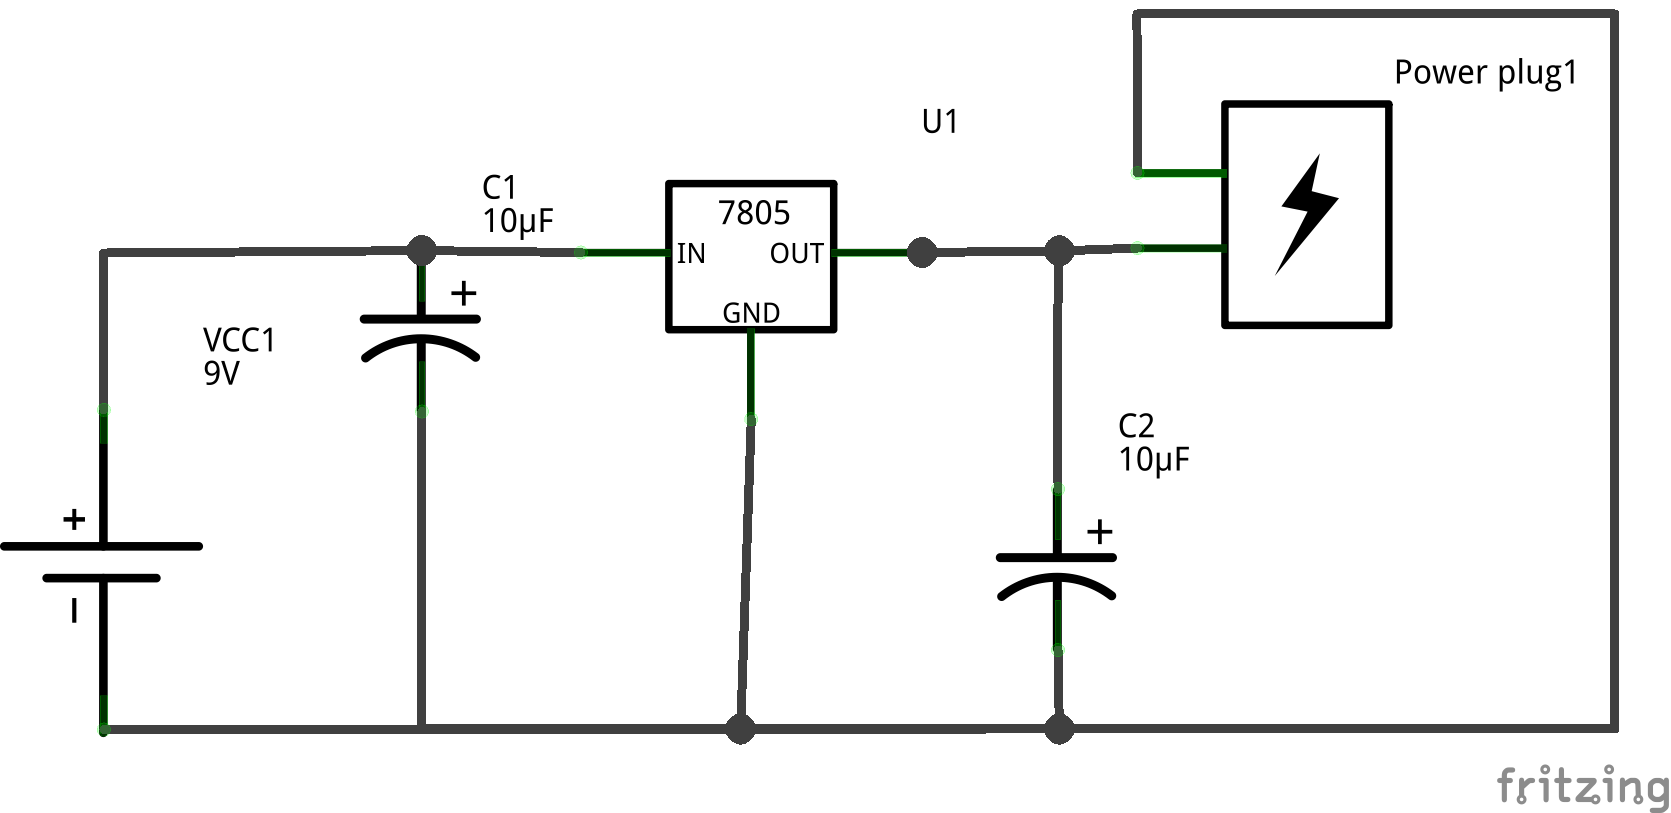
\includegraphics[width=4cm, height=4cm]{img/esquematrans.png}  & 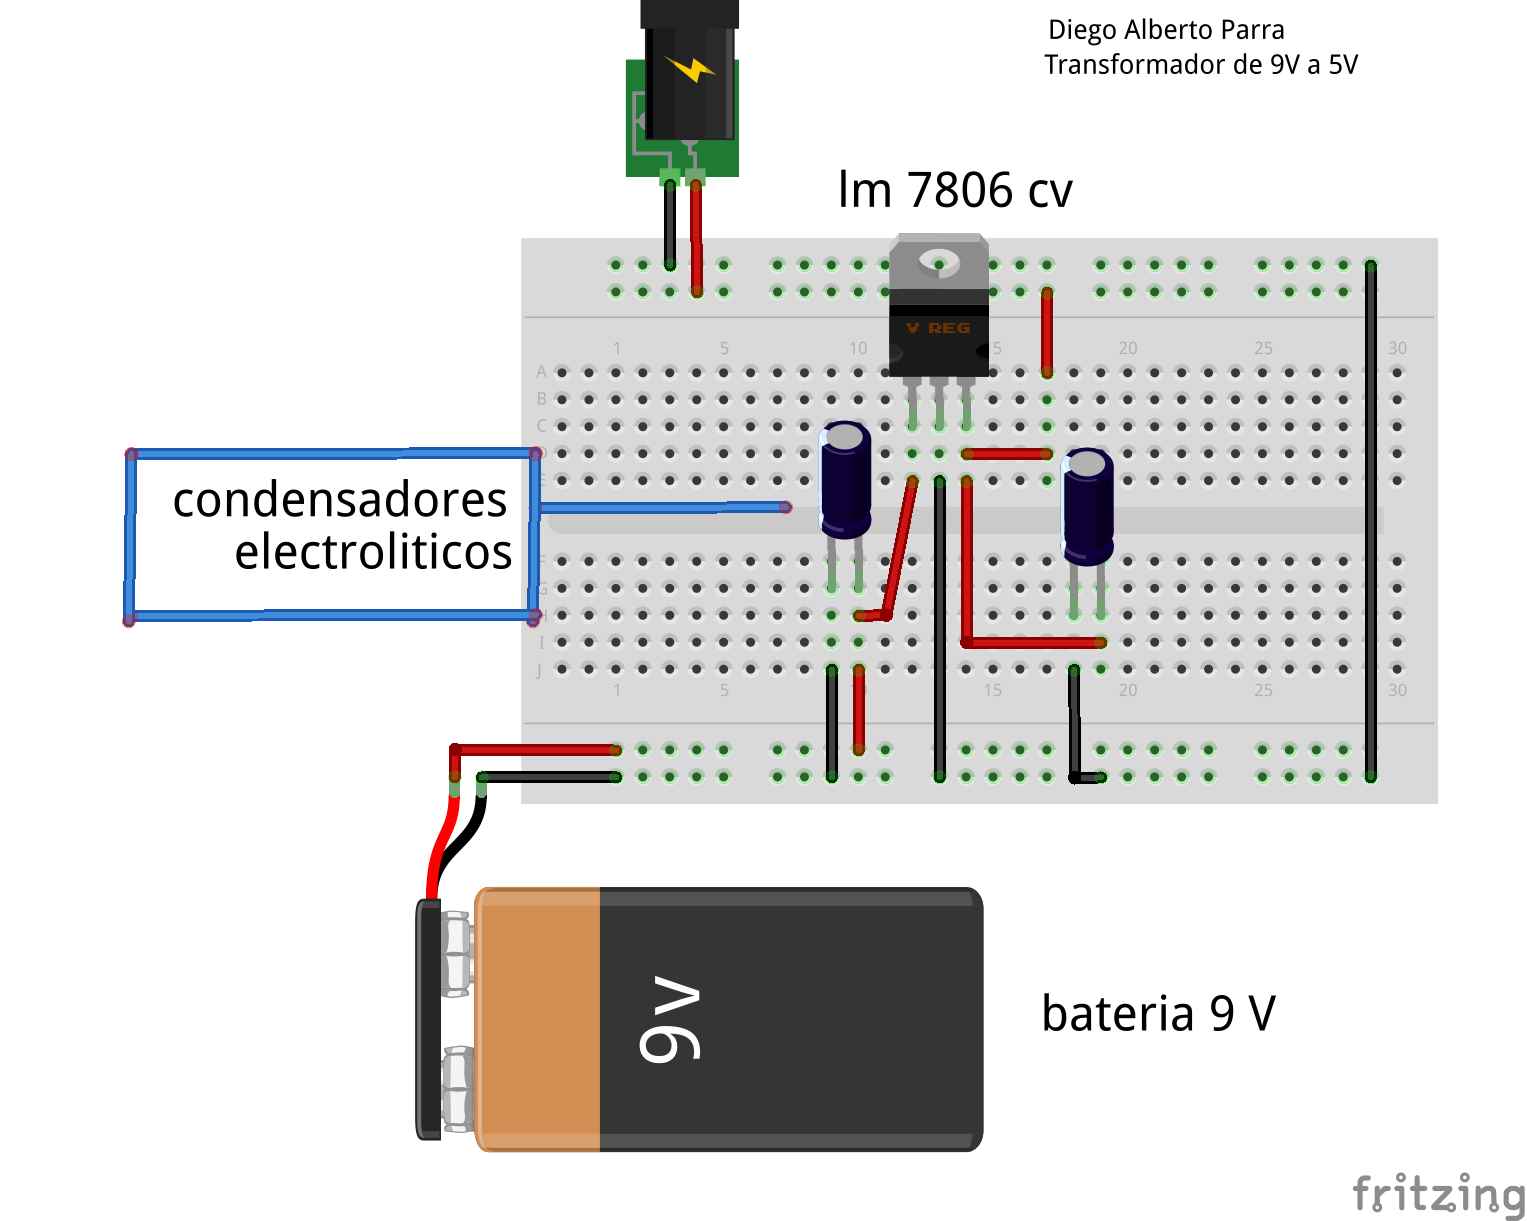
\includegraphics[width=4.cm, height=4cm]{img/montajetr5V.png} \\ \hline
1.A. & 1.B \\ \hline
\end{tabular}
\captionof{figure}{En la figura 1.A. se observa el esquema eléctrico de un transformador \cite{REGULADOR} de 9V a 5V, utilizando un transistor lm 7805 cv. Los capacitores son electrolíticos de 10 microfaradios.  En la figura 1.B. se observa el montaje en protoboard del circuito regulador.}
\label{fig:g1}
\end{Figure}
\vspace{0.2cm}

Montamos un transformador de 9 voltios a 5 voltios, esto lo hacemos con dos capacitores electrolíticos de 10 microfaradios  y el transistor lm7805\cite{REGULADOR} cv. Ambos  capacitores deben ir en paralelo quedando su extremo negativo conectado a tierra y su extremo positivo uno a la entrada de 9 V y el otro a la salida de 5 V del transistor, el transistor lm consta de 3 pines uno de los cuales es la entrada de +9V, el pin de la mitad es tierra o GND y el pin extremo es la salida a 5V; tal como se muestra en la figura 1.A.; en la figura 1.B. se le coloco un enchufe de salida de poder.
El modulo bluetooth se debe conectar de la siguiente manera: el pin 2 de la tarjeta arduino es el Rx este va conectado al Tx del blueetooth, el pin 3 del microcontrolador es el Tx y va conectado al pin Rx del bluetooth, como se muestra en la figura 2.A y 2.B , conectamos el GND del bluetooth al pin 8  o 16 de nuestro microcontrolador , ahora conectamos el pin de Vcc del bluetooth al pin 7 o 14 del microcontrolador. \\\\
Necesitamos colocar un oscilador de 16 mHz el cual lo dejaremos siempre en el microcontrolador, esto  con el fin de ajustar los tres relojes internos que trae nuestro integrado atmega 328 P-Pu, para esto utilizamos el cristal de 16 mHz junto con los dos condensadores cerámicos de 12 picofaradios \footnote{Ver figura 2.A y 2.B.}, uno de los pines del cristal debe conectarse al pin 9 del microcontrolador y el otro extremo del cristal al pin 10, conectamos un capacitor a cada extremo del cristal y estos al pin 8 o 16 del microcontrolador de tal forma que los capacitores quedan en paralelo. \\\\
Colocamos un botón\footnote{Como se muestra en la figura 2.A y 2.B.} para reiniciar nuestro microcontrolador en caso de que lo necesitamos, esto lo hacemos colocando uno de los extremos del botón al pin 1 del microcontrolador que es el pin de reset, el otro extremo del botón lo conectamos a una resistencia de 1 Komhs y el extremo de la resistencia a tierra.\\\\

\begin{Figure}
\center
\begin{tabular}{|l|r|}
\hline
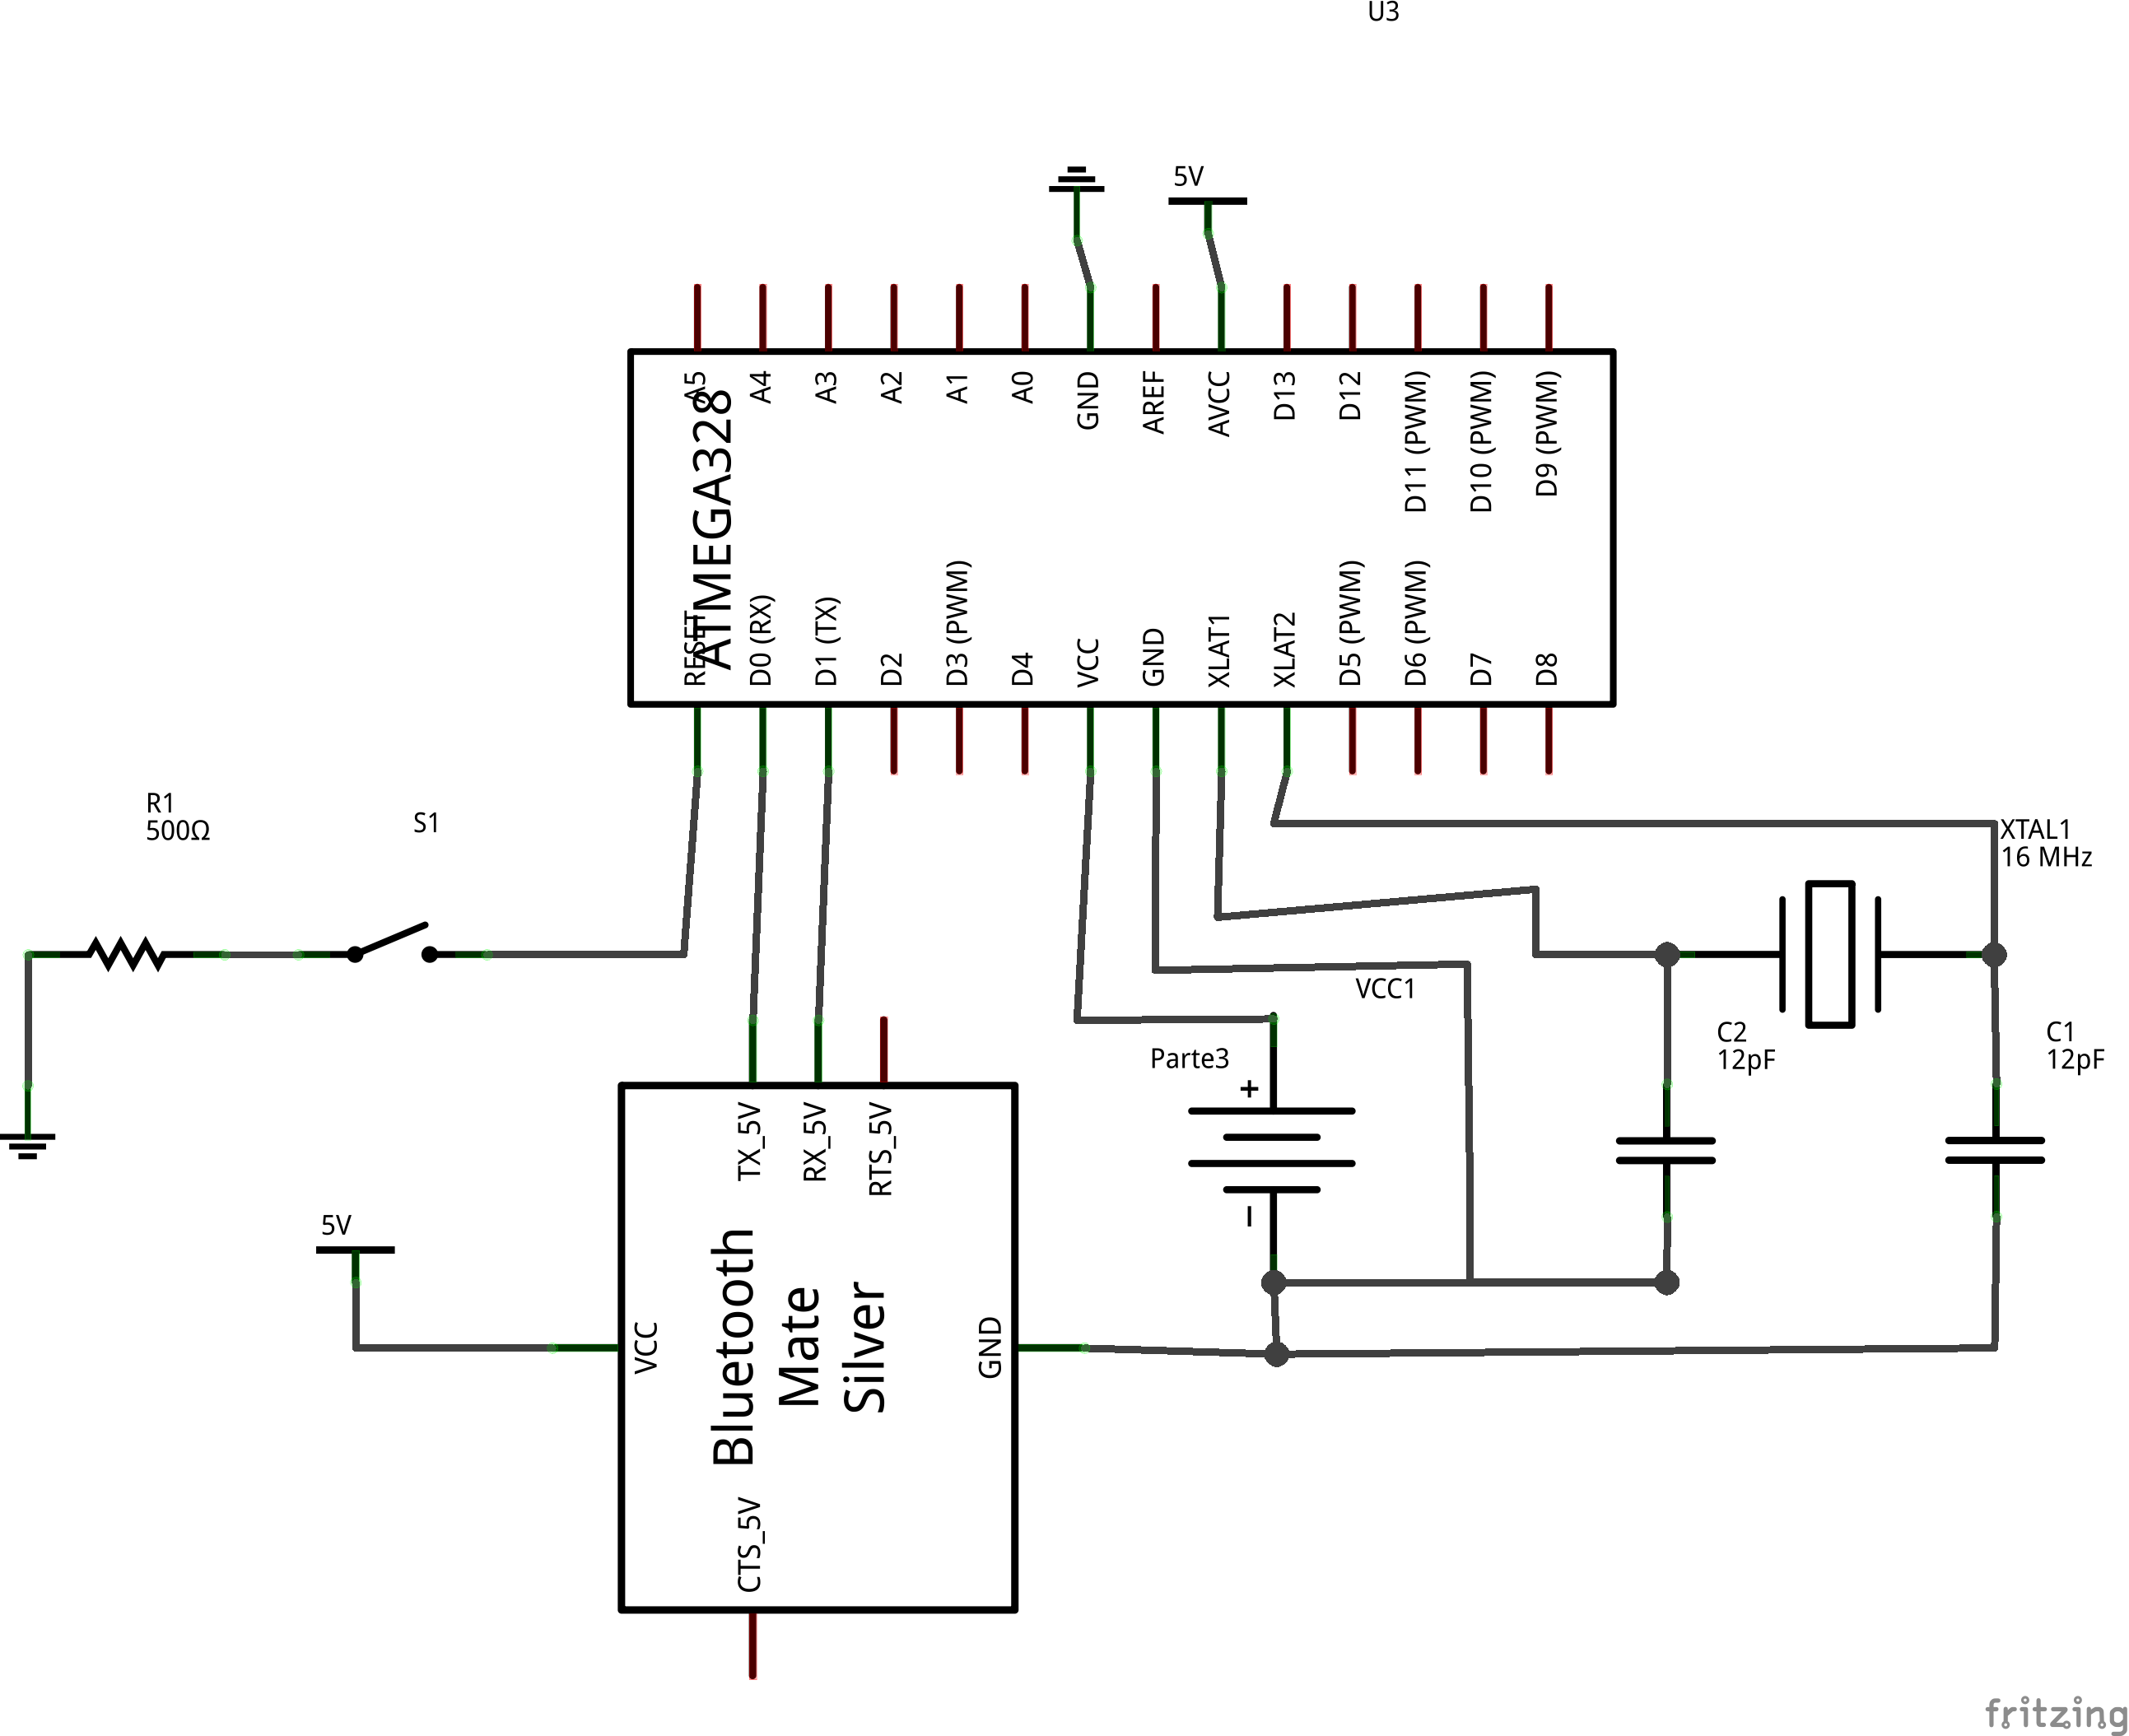
\includegraphics[width=4cm, height=4cm]{img/bluetoothesq.png} & 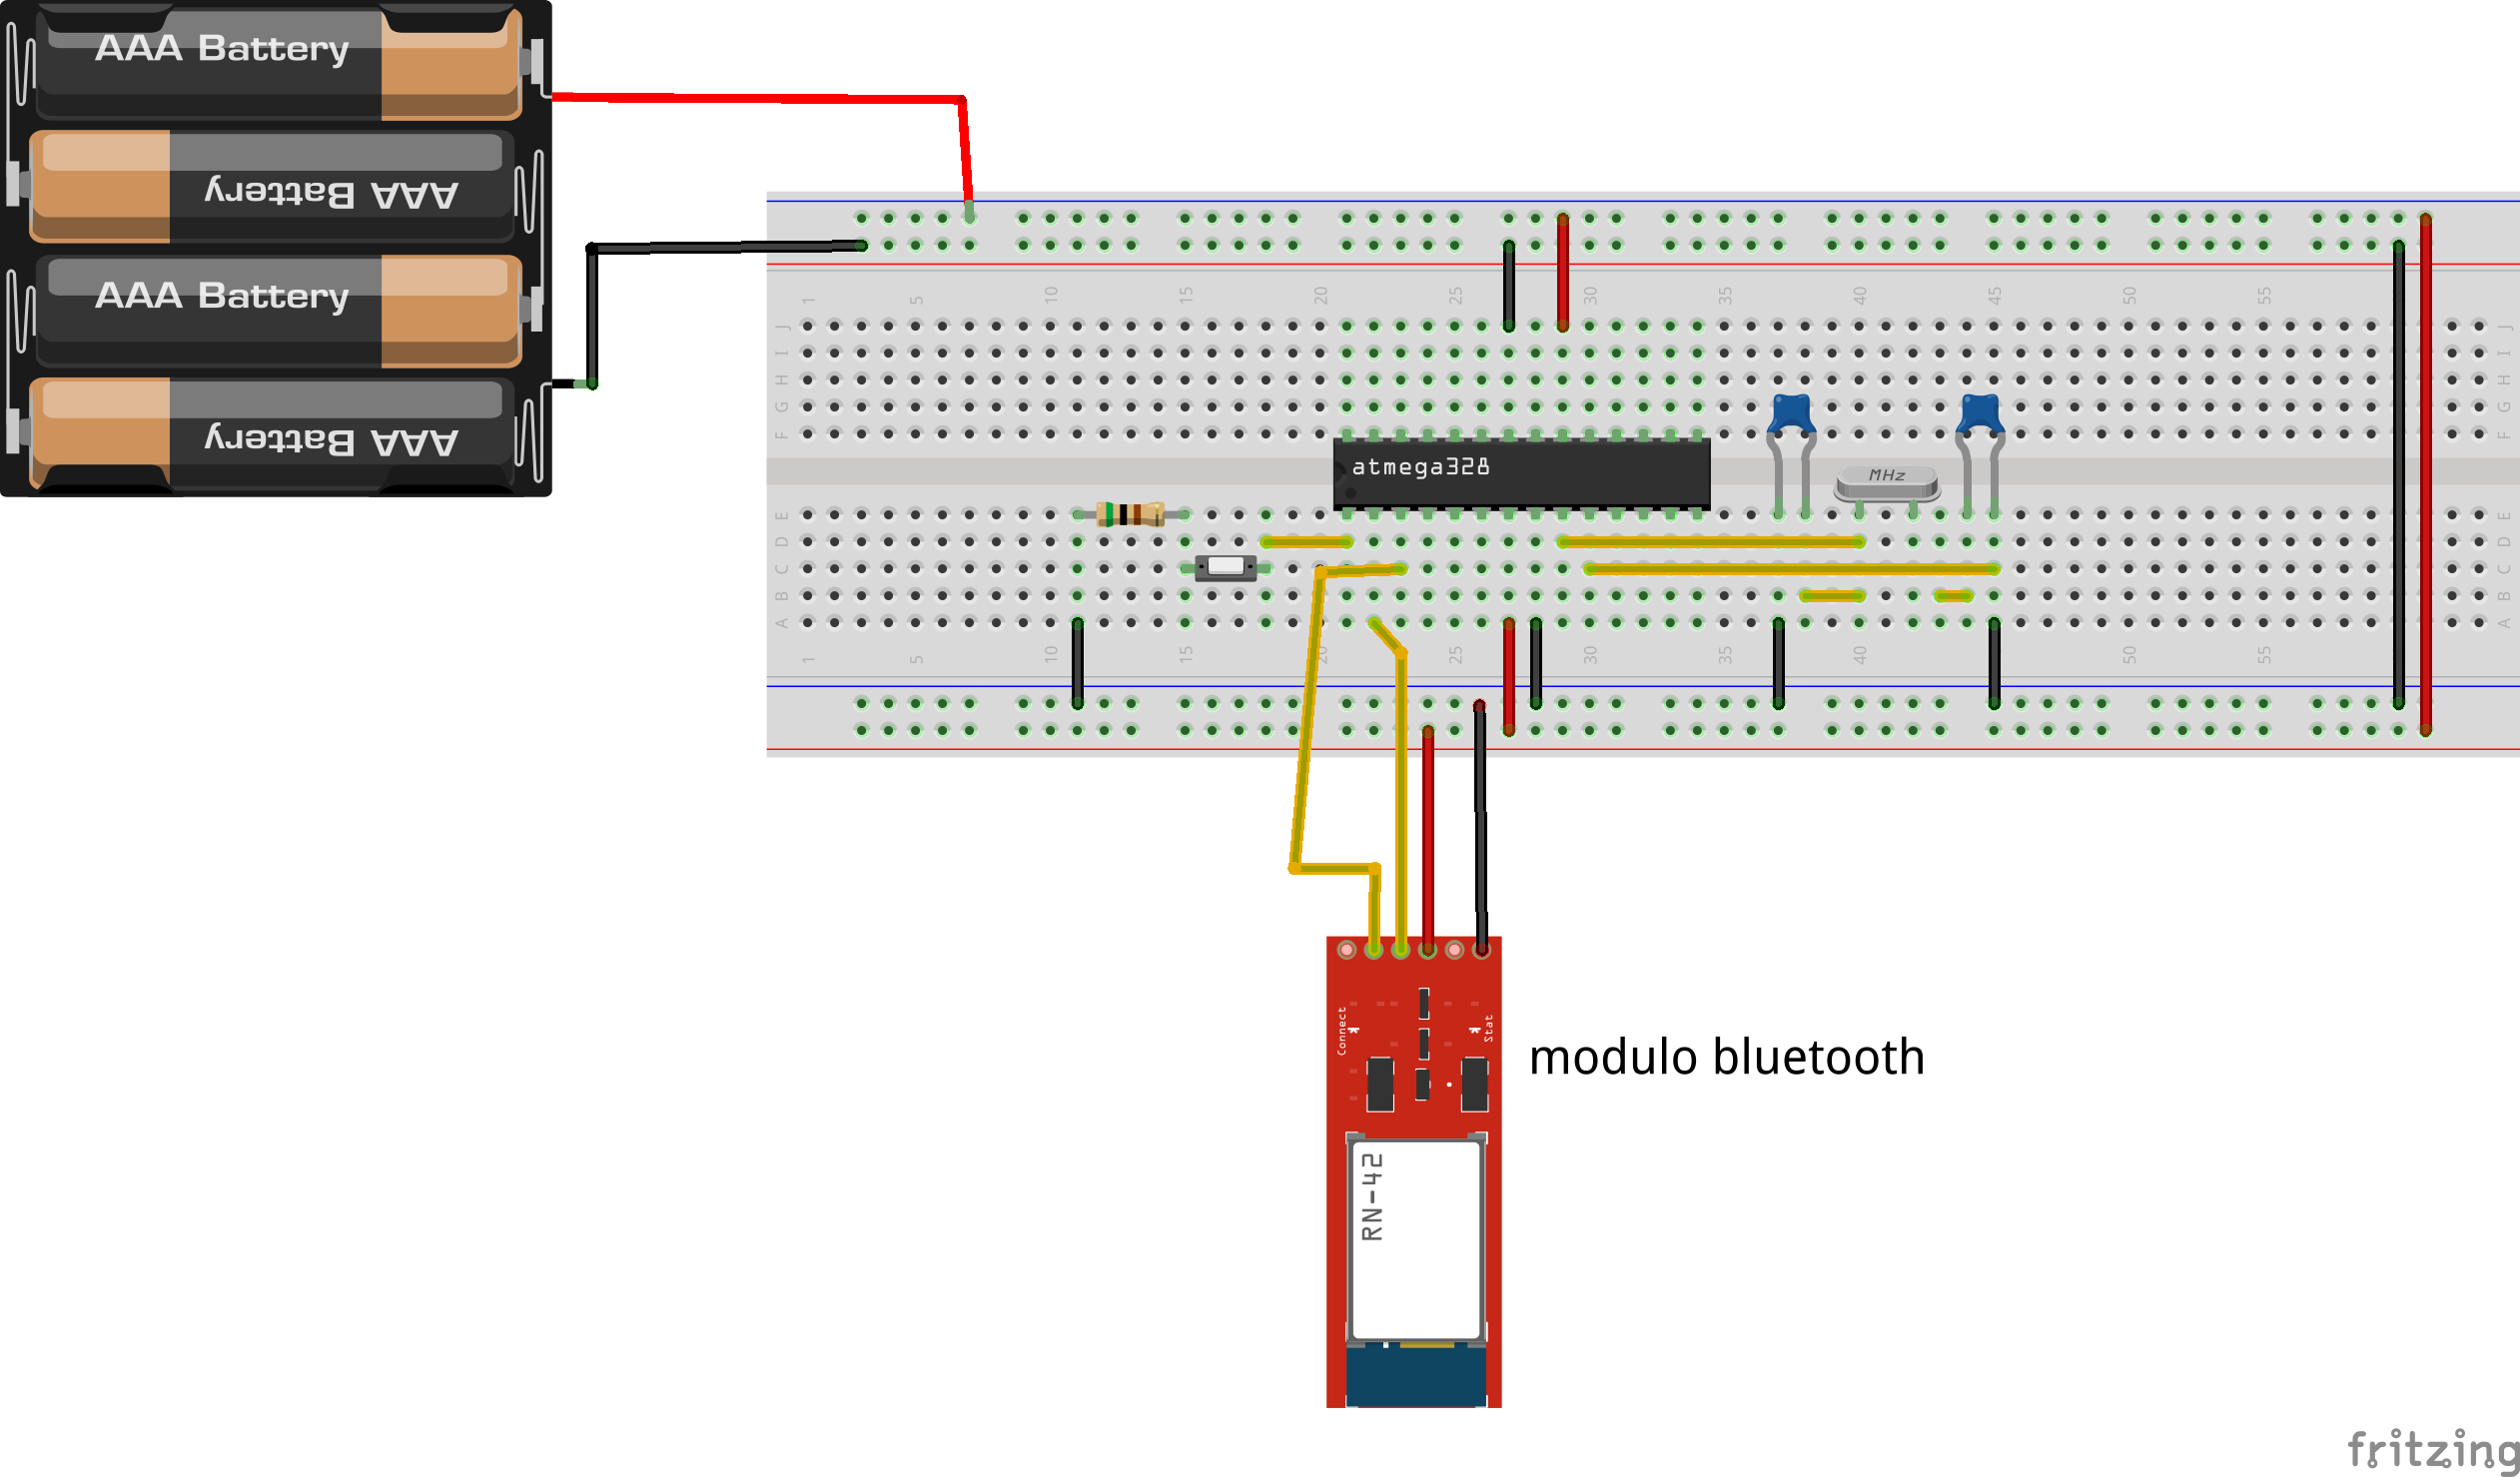
\includegraphics[width=4cm, height=4cm]{img/bluetoothmon.png} \\ \hline
2.A. & 2.B. \\ \hline
\end{tabular}
\captionof{figure}{En la figura 2.A se muestra el circuito eléctrico de un bluetooth conectado a un microcontrolador atmega 328 P-PU junto con un cristal, dos capacitores cerámicos, un botón de reset y una resistencia de 1 Komhs. En la figura 2.B esta  el montaje en protoboard, los cables negros son tierra, los cables rojos son voltaje, y los cables amarillos son conexiones.}
\label{fig:g2}
\end{Figure}
\vspace{0.2cm}

Las conexiones del motor son las siguientes, como vamos a utilizar un transistor tip\cite{TIP122} 122, los pines mostrados en la figura 2.B.  están de la siguiente manera: 

\begin{enumerate}
\item[*] El pin del lado izquierdo del transistor es la base.
\item[*] El pin del centro es el colector.
\item[*] El pin de la derecha es el emisor.
\end{enumerate}

Conectamos una resistencia de 1 $k \Omega $ al pin base del transistor y este a su vez al pin numero 5 del integrado atmega328P-PU\footnote{Como se aprecia en la figura 2.B.}, luego conectamos el pin del colector del tip122 a +5V, asegurándonos de colocar el diodo regulador entre el colector y uno de los extremos del motor; a continuación conectamos el pin emisor del transistor  junto con el otro extremo de la conexión del motor a tierra; ahora colocamos las conexiones del condensador cerámico entre las conexiones del motor.\footnote{Observar figuras 2.A. y 2.B.}


\begin{Figure}
\center
\begin{tabular}{|l|r|}
\hline
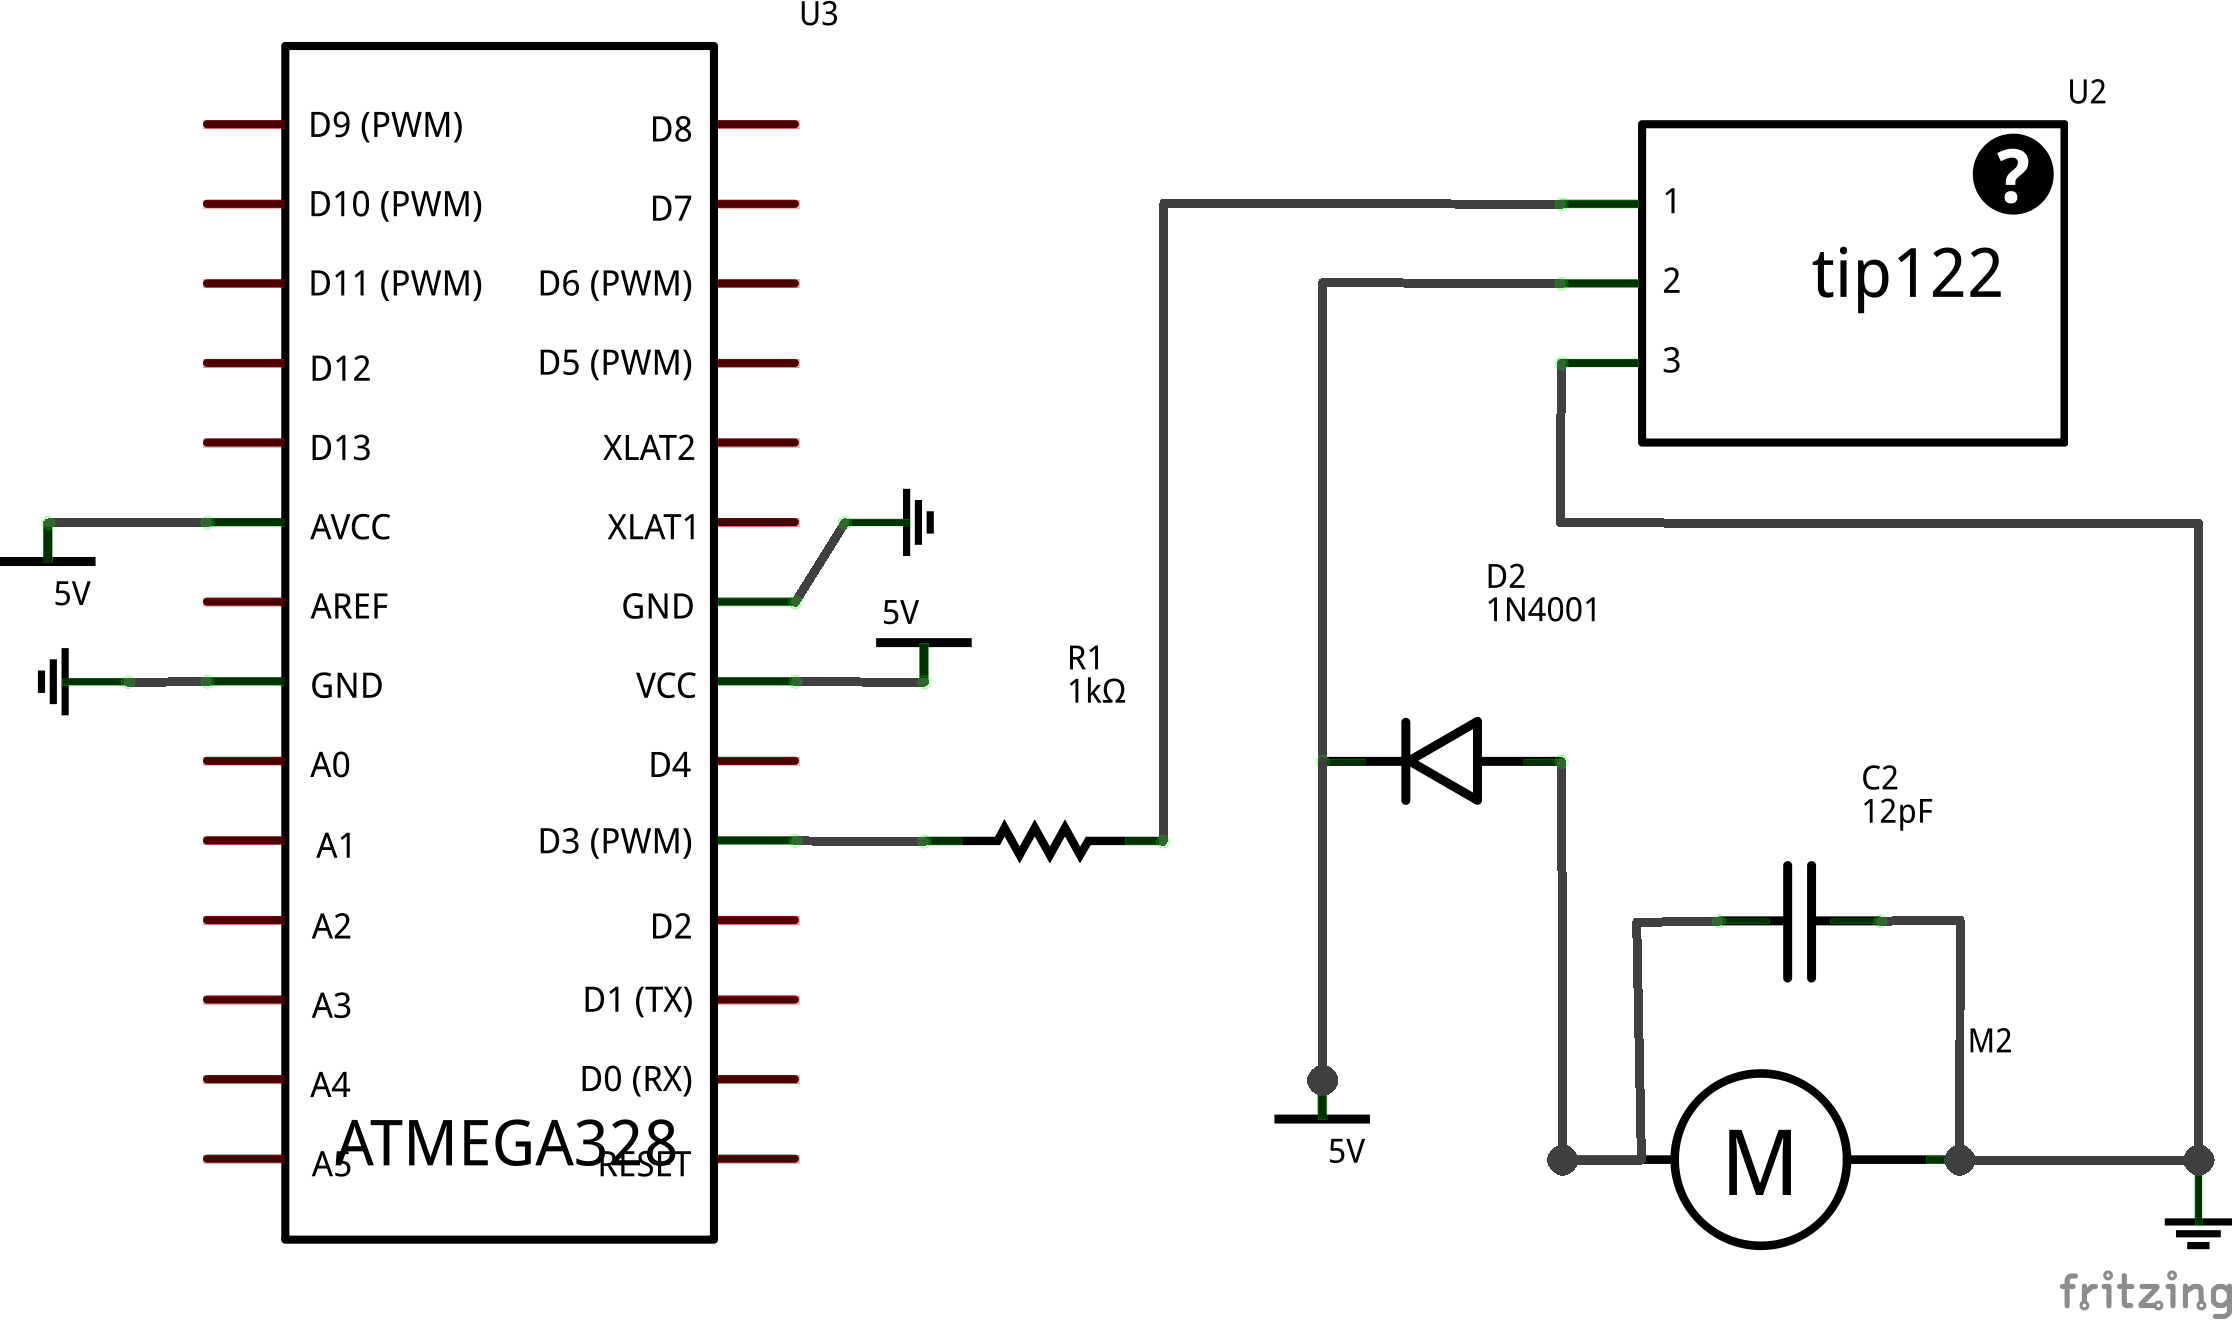
\includegraphics[width=4cm, height=4cm]{img/esquemamotor.png} & 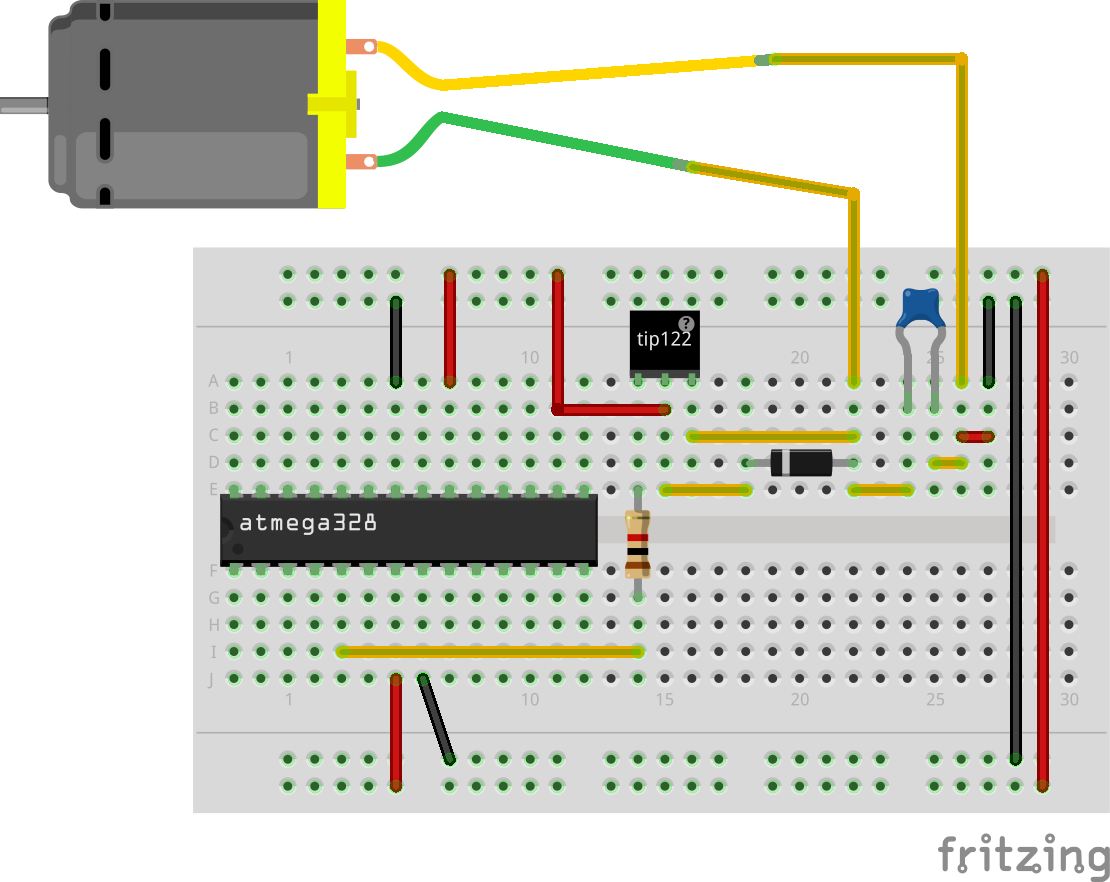
\includegraphics[width=4cm, height=4cm]{img/montajemot.png} \\ \hline
3.A. & 3.B. \\ \hline
\end{tabular}
\captionof{figure}{En la figura 3.A se muestra el circuito eléctrico del motor conectado a la tarjeta atmega 328 P-PU, junto con un tip 122 encargado de controlar la corriente que circula por el  motor consiguiendo de esta manera controlar la velocidad de este, también lleva un diodo regulador, un capacitor cerámico de  12 picofaradios y una resistencia de 1 Komhs. En la figura 3.B esta  el montaje en protoboard, los cables negros son tierra, los cables rojos son voltaje, y los cables naranjas son conexiones.}
\label{fig:g3}
\end{Figure}

Procedemos hacer las conexiones del sensor receptor lateral \footnote{Se aprecia en la figura 4.A. y en la figura 4.B.} el cual es un diodo led receptor de luz infrarroja \cite{INFRARED}, conectamos una resistencia de $1 k\Omega$ al ánodo del led y el otro extremo de la resistencia a tierra, luego conectamos el pin 28 \footnote{Este pin es la entrada analógica numero cero del microcontrolador atmega.} del microcontrolador en un punto intermedio entre la resistencia y el ánodo del diodo led, el cátodo del diodo lo conectamos a +5V.\\\\
Para las conexiones del sensor receptor frontal \footnote{Se aprecia en la figura 4.A. y en la figura 4.B., en la parte donde están los dos diodos led.} el cual es un diodo led receptor de luz infrarroja \cite{INFRARED}, conectamos una resistencia de $1 k\Omega$ al ánodo del led y el otro extremo de la resistencia a tierra, luego conectamos el pin 22 \footnote{Este pin es la entrada analógica numero cinco del microcontrolador atmega.} del microcontrolador en un punto intermedio entre la resistencia y el ánodo del diodo led, el cátodo del diodo lo conectamos a +5V.\\\\
Para la conexión de la fuente\footnote{Ver figura 4.B. y su esquema en la figura 4.A.} emisora de fotones infrarrojos o radiación infrarroja se utiliza un diodo led emisor en el infrarrojo, el cátodo del diodo lo conectamos a una resistencia de $350 \Omega$ a $500 \Omega$ y el otro extremo de la resistencia lo conectamos a tierra, el ánodo del diodo lo conectamos al pin 12\footnote{Salida D6 PWM.} del microcontrolador.

\begin{Figure}
\center
\begin{tabular}{|l|r|}
\hline
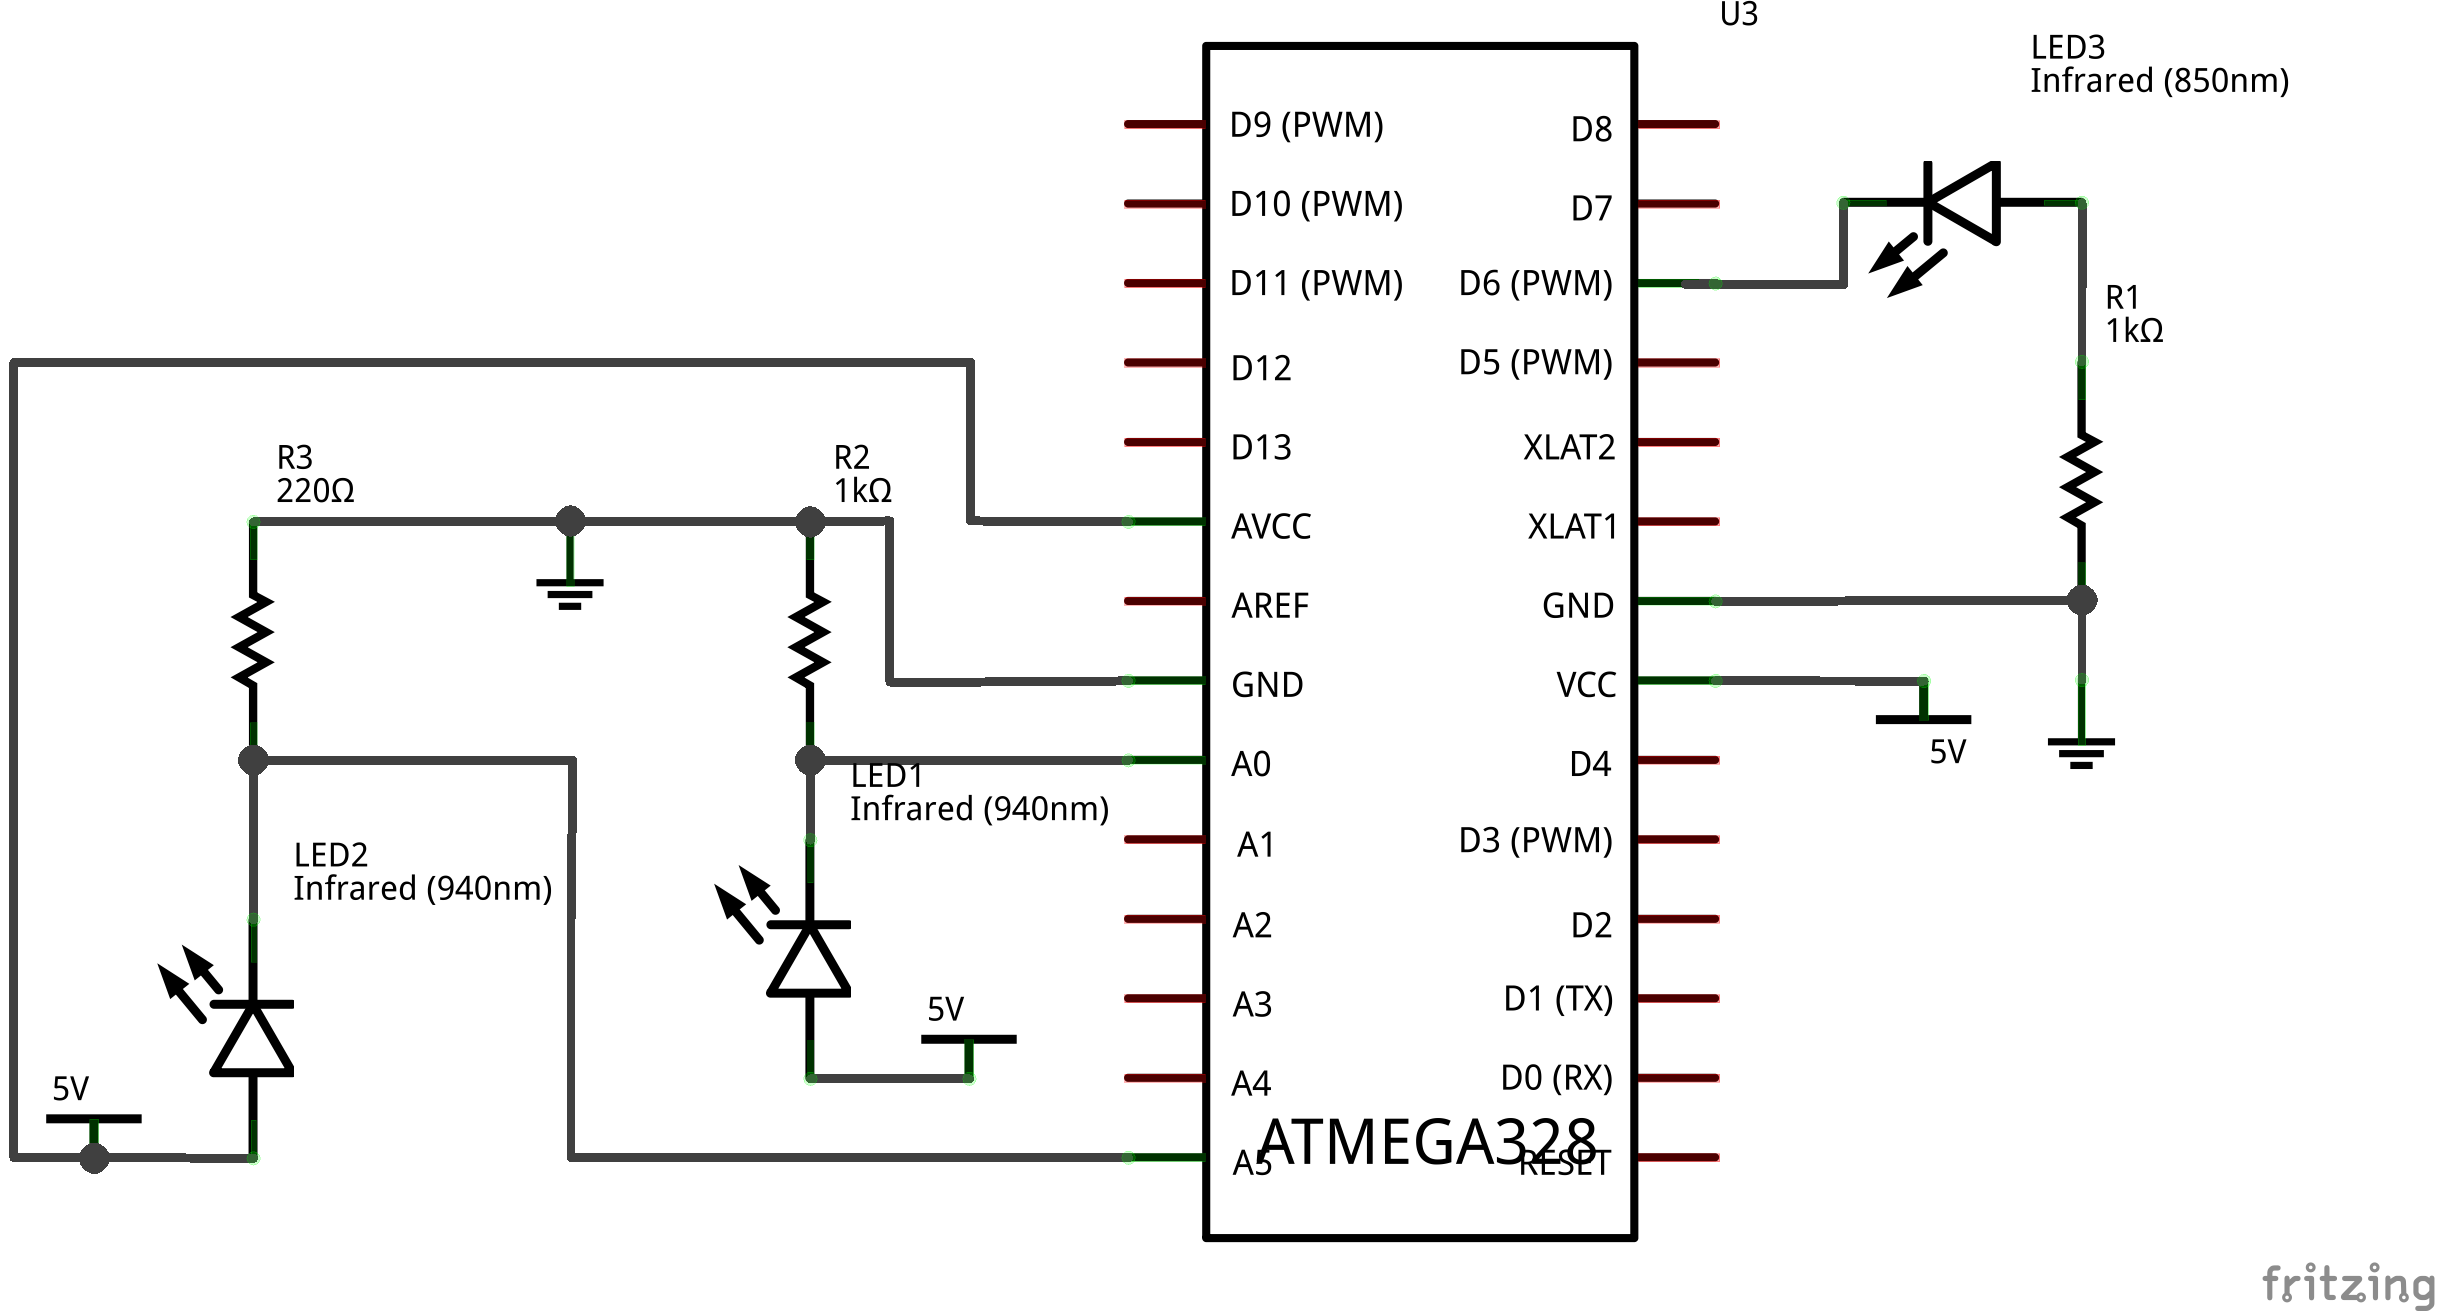
\includegraphics[width=4cm, height=4cm]{img/ledesq.png} & 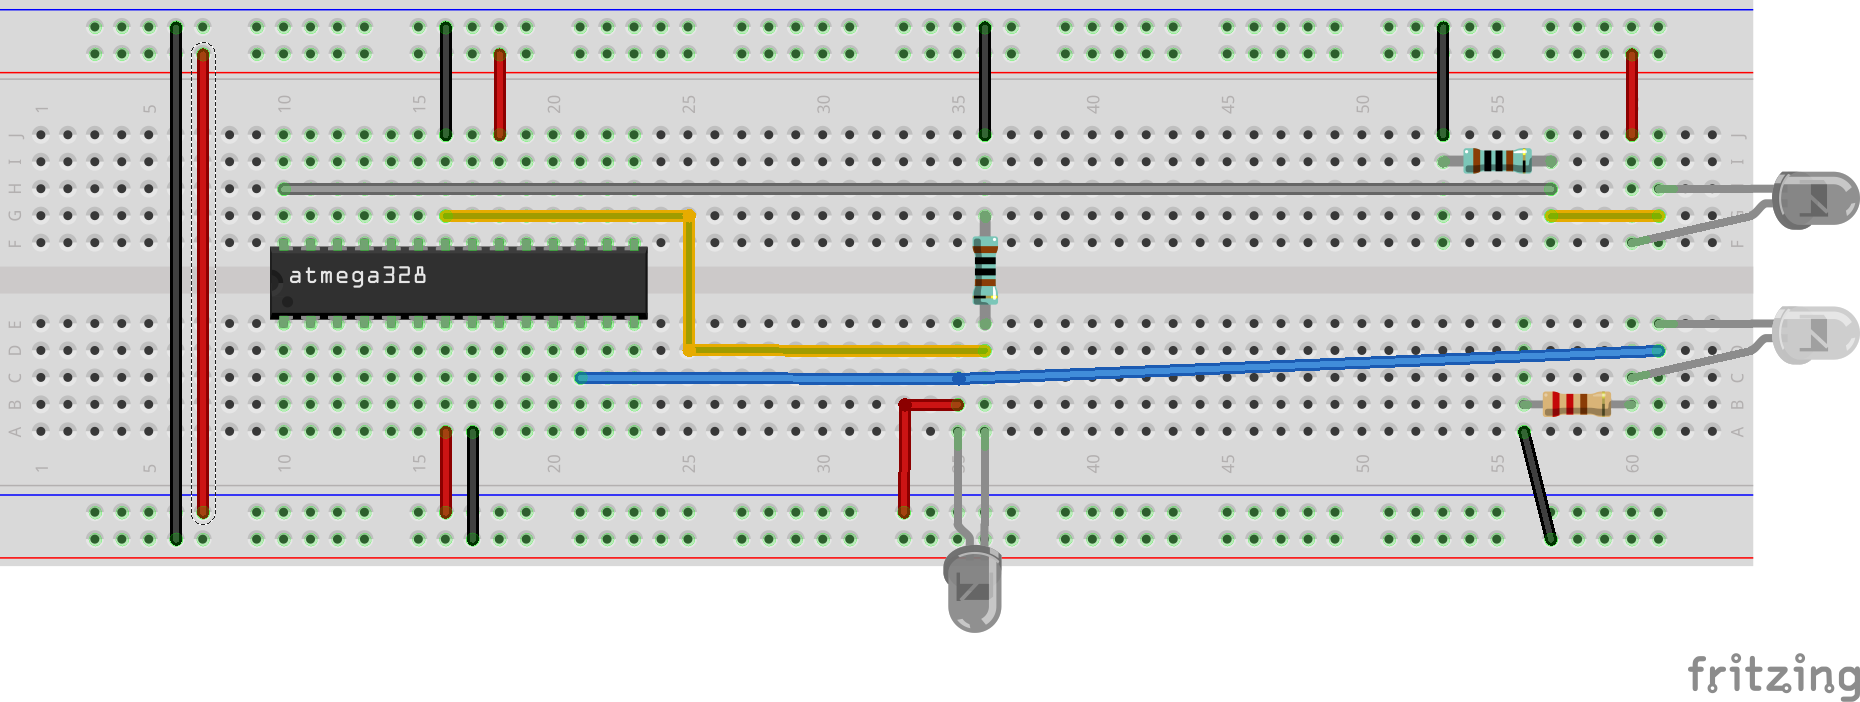
\includegraphics[width=4cm, height=4cm]{img/ledmont.png} \\ \hline
4.A. & 4.B. \\ \hline
\end{tabular}
\captionof{figure}{En la figura 4.A se observa las conexiones de los diodos tanto receptores como el emisor, conectamos al microcontrolador atmega328P-PU. En la figura 4.B esta  el montaje en protoboard, los cables negros son tierra, los cables rojos son voltaje, el cable azul es la conexión entre el ánodo del diodo led emisor infrarrojo frontal y el pin 6 del microcontrolador, el cable naranja es la conexión entre el pin 23 del microcontrolador y el punto de conexión entre el ánodo del  diodo receptor infrarrojo lateral con la resistencia, el cable gris  es la conexión entre el pin 28 del microcontrolador y el punto de conexión entre el ánodo del diodo receptor infrarrojo frontal con la resistencia.}
\label{fig:g4}
\end{Figure}

Las conexiones\footnote{Ver los esquemas de la figura 5.A. y 5.B.} del diodo rgb de ánodo común es la siguiente: conectamos el ánodo del diodo rgb a +5V, el pin rojo del diodo rgb lo conectamos a una resistencia de $500\Omega$ y el otro extremo de la resistencia conectado al pin 18 del microcontrolador, el pin verde del diodo rgb lo conectamos a una resistencia de $500\Omega$ y el otro extremo de la resistencia conectado al pin 16 del microcontrolador, el pin azul del diodo rgb lo conectamos a una resistencia de $500\Omega$ y el otro extremo de la resistencia conectado al pin 15 del microcontrolador.\\\\
Una vez terminadas las conexiones solo resta soldarlas en una baquela. Por ultimo pero no menos importante es conseguir icopor y hacer unas bases para que en ellas repose nuestro circuito de esta manera nos aseguramos en caso de cualquier incidente que las placas no se vayan a estropear ni que las conexiones vayan a quedar haciendo corto.
\begin{Figure}	
\center
\begin{tabular}{|l|r|}
\hline
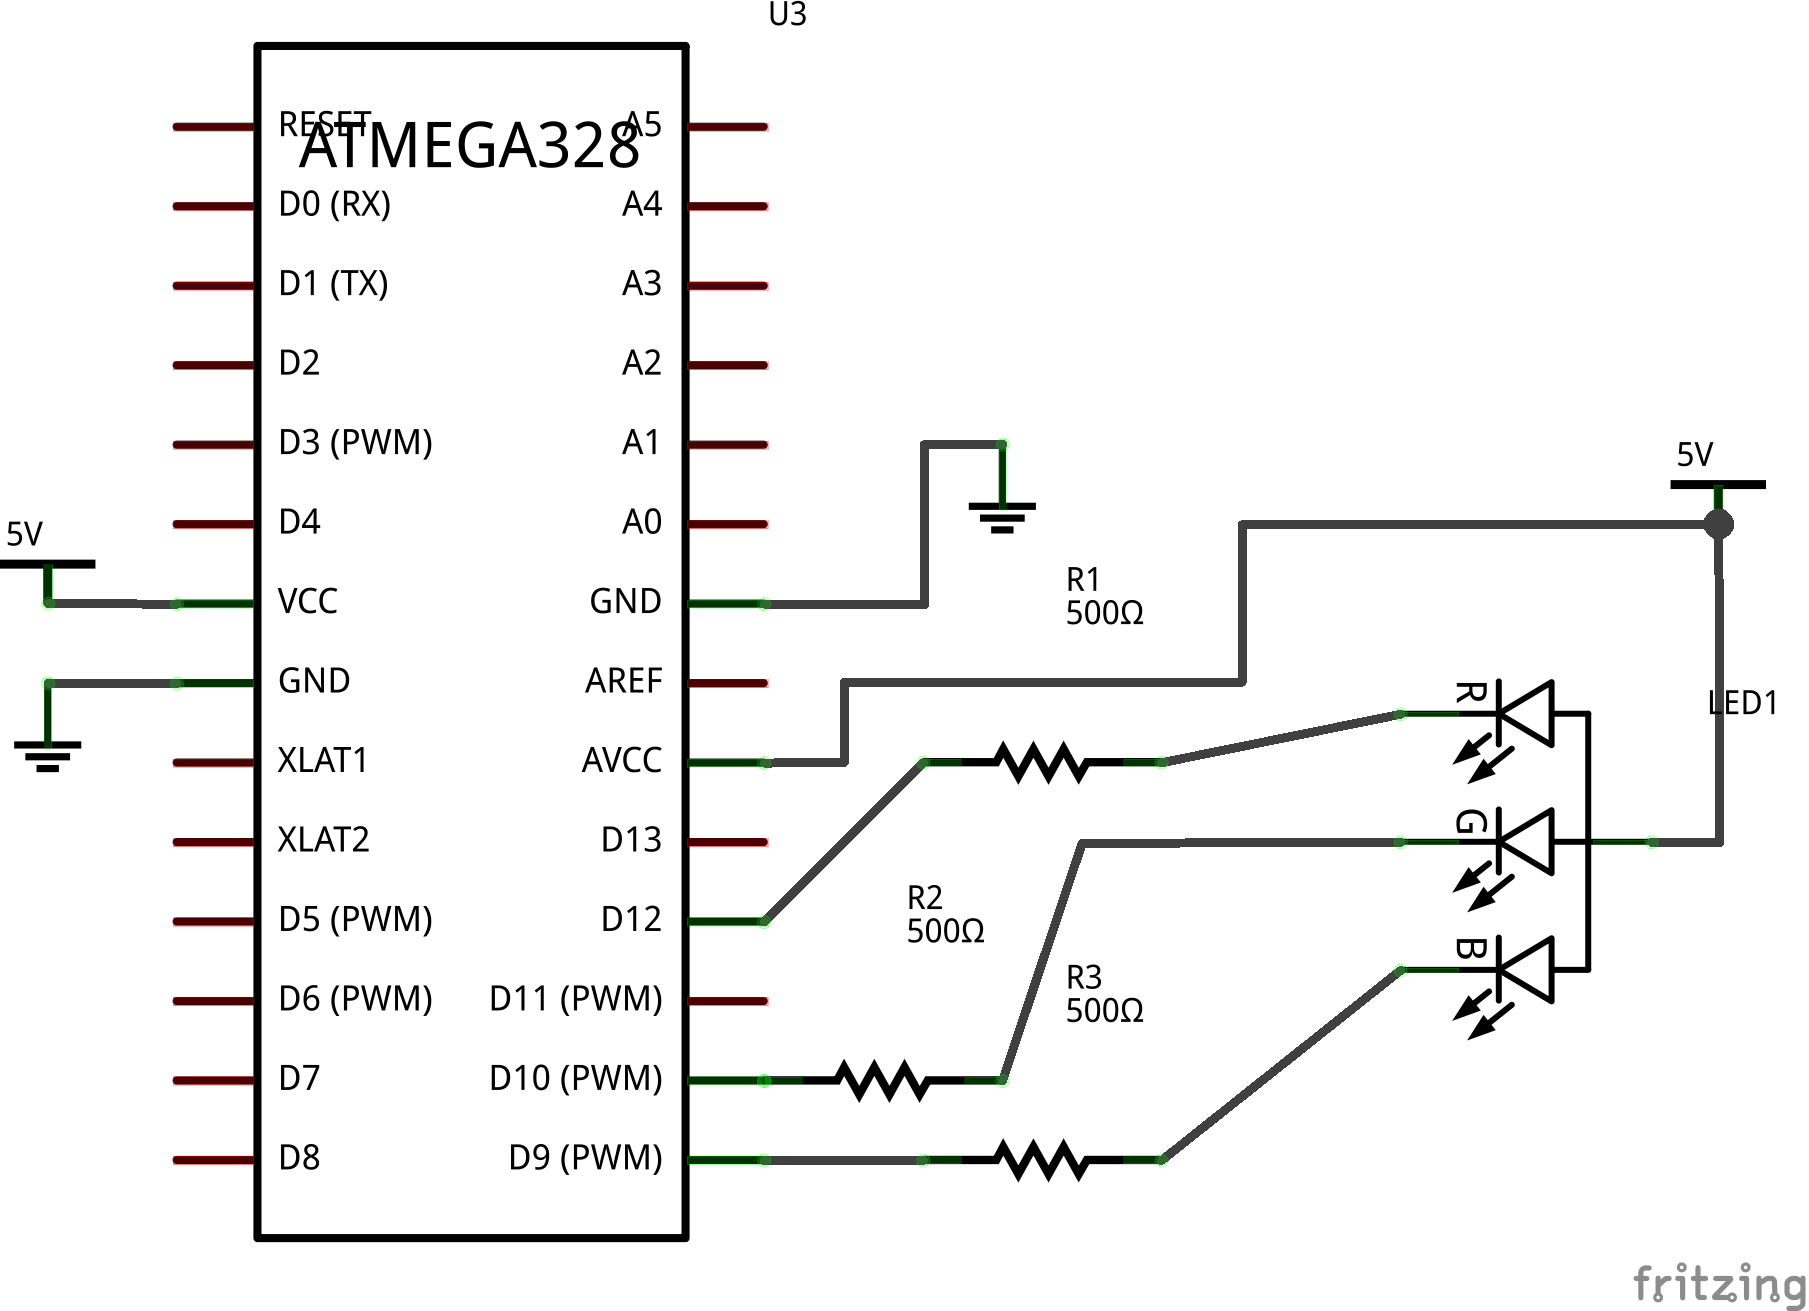
\includegraphics[width=4cm, height=4cm]{img/rgbesq.png} & 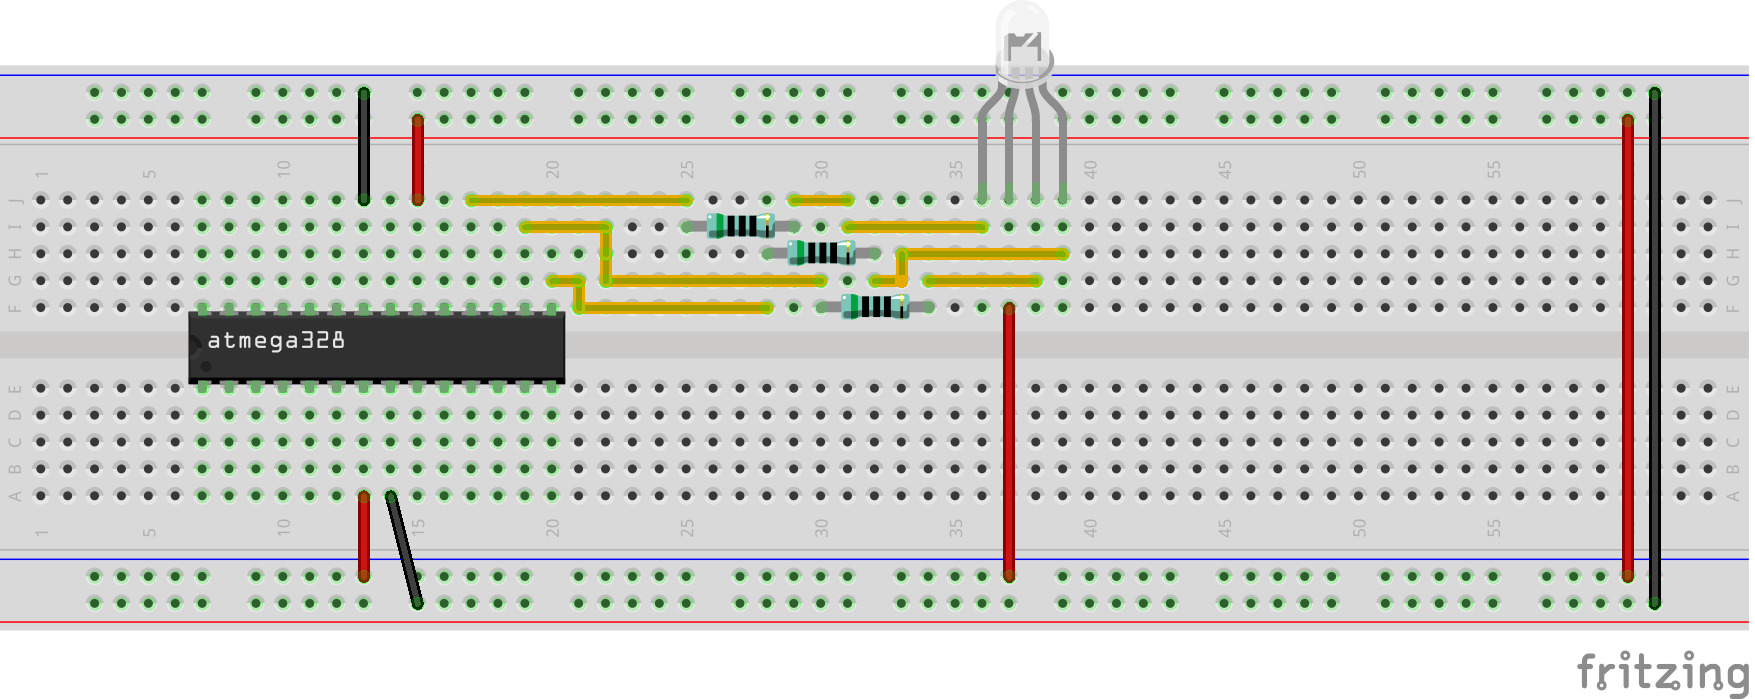
\includegraphics[width=4cm, height=4cm]{img/rgbmont.png} \\ \hline
5.A. & 5.B. \\ \hline
\end{tabular}
\captionof{figure}{En la figura 5.A. se muestra el circuito eléctrico del diodo rgb conectado al microcontrolador atmega 328 P-PU. En la figura 5.B esta  el esquema  del diodo rgb en protoboard.}
\label{fig:g5}
\end{Figure}
\vspace{0.6 cm}

Esa era la parte eléctrica ahora los esquemas eléctricos deben unirse para formar un solo circuito\footnote{Ver figura 6.A., y 6.B.}, antes de soldar el microcontrolador atmega 328P-PU es necesario cargar el archivo de control del hardware, cuyos pasos son los siguientes:
\begin{enumerate}
\item[a.] Instalar git \footnote{Enlace para instalar git  http://git-scm.com/download/linux }
\item[b.] Descargar el repositorio de este proyecto \footnote{En una terminal escribimos git  clone https://github.com/Diego-debian/Modulo\_Motorizado.git}.
\item[c.] Una vez descargado el repositorio hay que ir desde la terminal de linux a la carpeta donde se encuentra alojado el repositorio que acaba de descargar; si usted clono el repositorio en su carpeta home, solo coloque la siguiente linea en una terminal  sin la primera y ultima comilla “cd "Modulo\_Motorizado/0. Instalación/0.1 programas requeridos/"”.
\item[d.] Acceda como usuario root y a continuación escriba en la terminal la siguiente linea sin las comillas “python install.py”, se abrirá el programa de instalación del proyecto, ahora siga las instrucciones del programa.
\item[e.] Al terminar el programa le pedira si desea reiniciar el ordenador, escriba n y luego presione enter.
\item[f.] Escriba sin las comillas “exit” y oprima enter, luego escriba “arduino” y oprima enter, abrirá una ventana donde debe seleccionar la opción add. Luego de esto vera la IDE de arduino, ciérrela y reinicie el ordenador.
\item[g.] Desde nuestro navegador de archivos del sistema\footnote{Puede estar utilizando los siguientes en su distribución linux, nautilus, thunar o algún otro.}  entramos a la carpeta Modulo\_Motorizado/1. Inicio/ 1.2 programar arduino y sensores, allí encontraremos el archivo sensores2.ino, lo seleccionamos y oprimimos enter.
\item[h.] Conectamos la tarjeta arduino junto con el microcontrolador que vamos a dejar en el proyecto, en la IDE de arduino vamos a la opción herramientas,  tarjeta y seleccionamos arduino uno;  ahora nuevamente en herramientas, damos click en puerto serial y seleccionamos el puerto que nos aparece,  ahora oprimimos la tecla ctrl y la tecla “u” \footnote{Sin las comillas.} al mismo tiempo y esperamos mientras carga el sketch, una vez cargado retiramos el microcontrolador y lo colocamos en la parte del proyecto donde se le dispuso su sitio.   
\end{enumerate}

\begin{Figure}	
\center
\begin{tabular}{|l|r|}
\hline
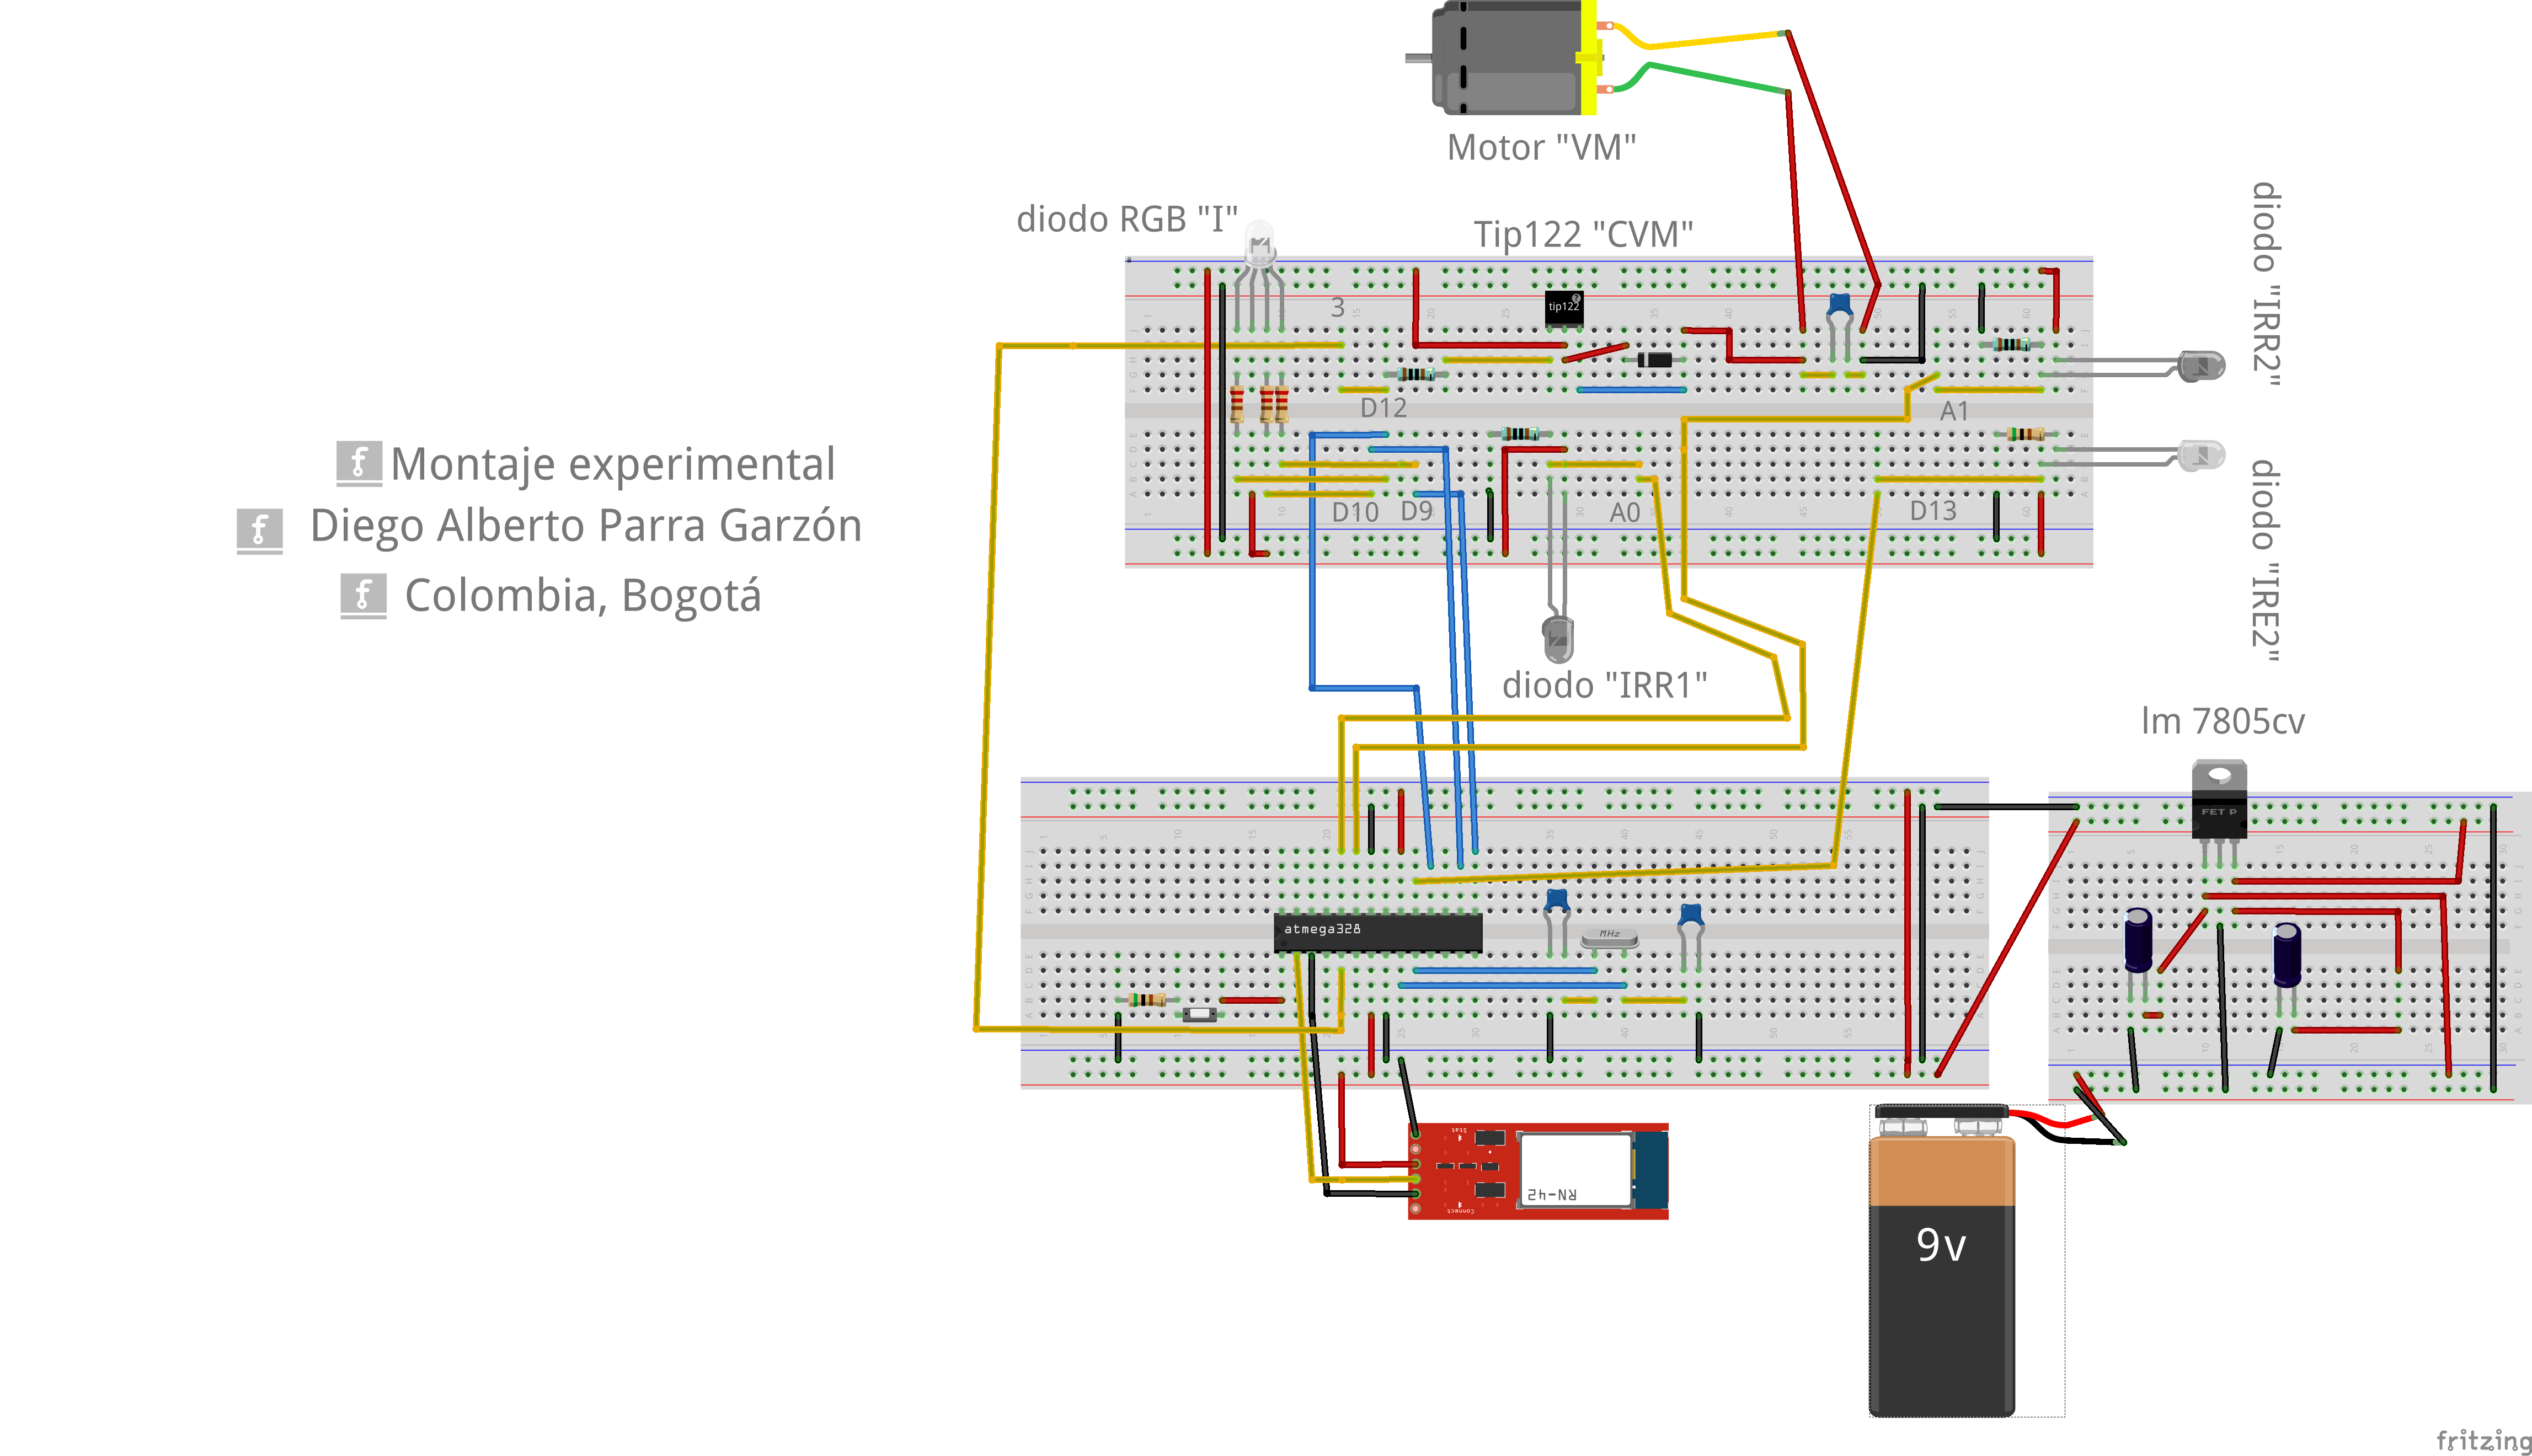
\includegraphics[width=4cm, height=4cm]{img/montajep.png} & 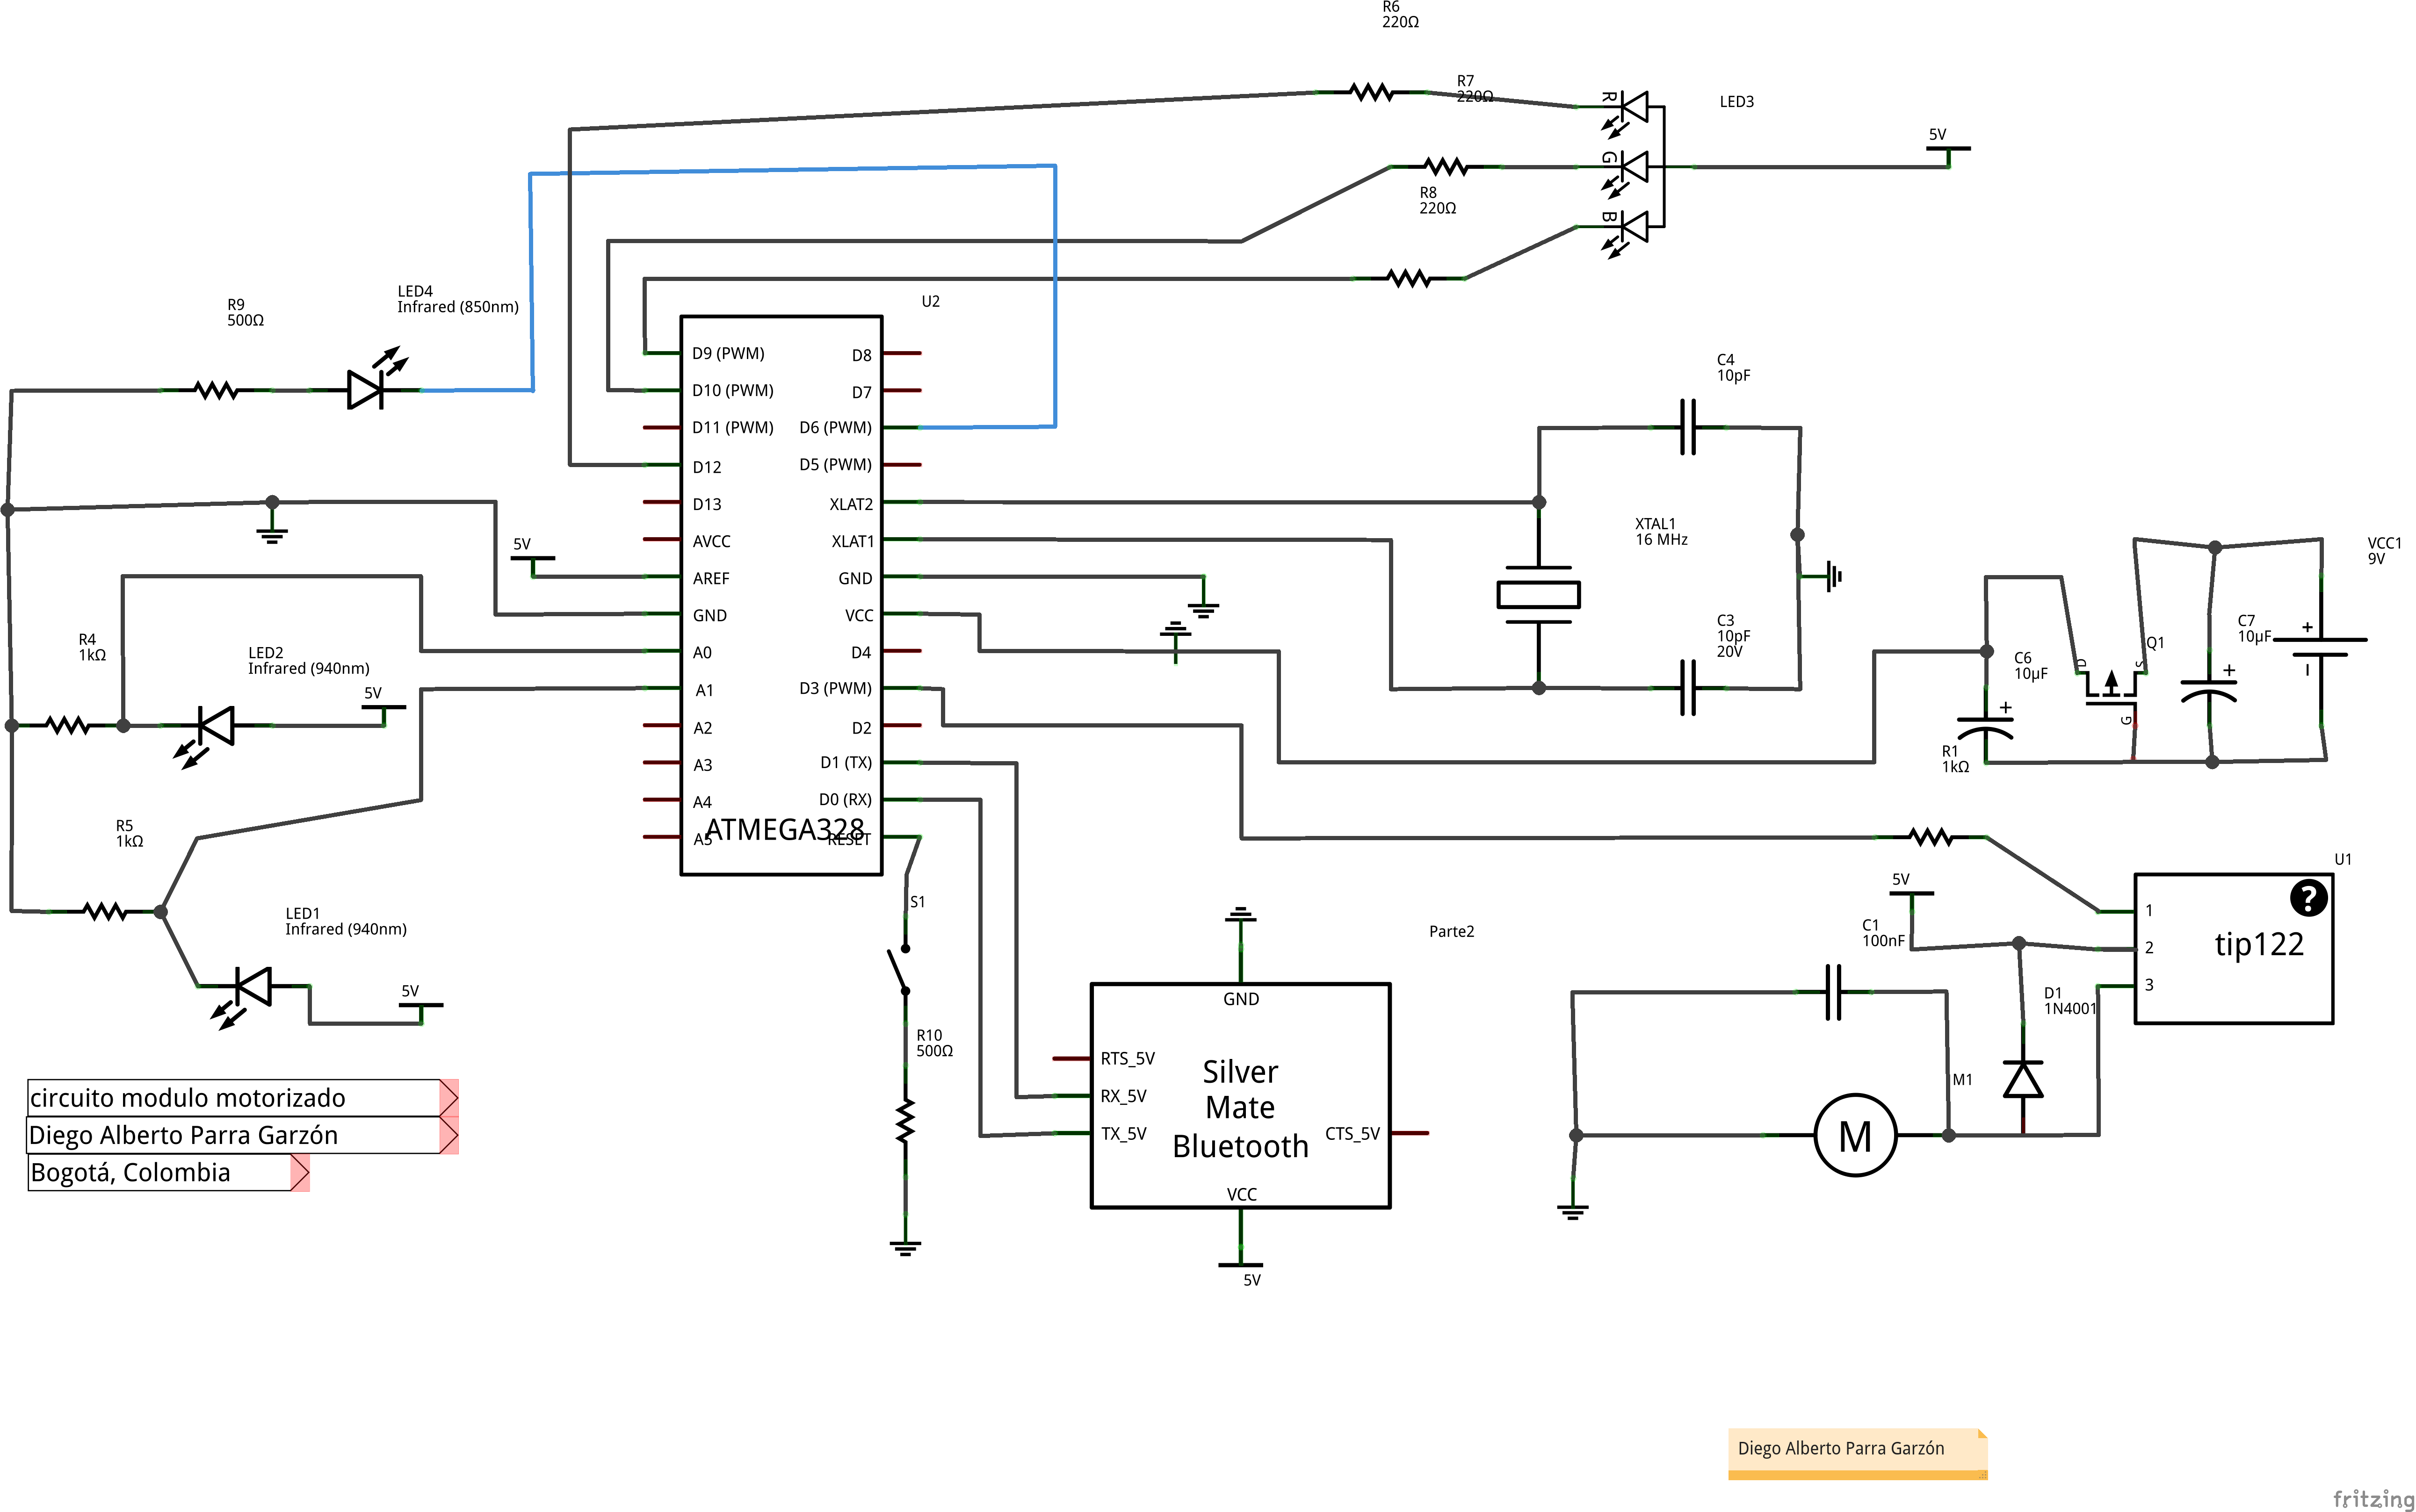
\includegraphics[width=4cm, height=4cm]{img/esquemap.png} \\ \hline
6.A. & 6.B. \\ \hline
\end{tabular}
\captionof{figure}{En la figura 6.A. se muestra el circuito eléctrico del proyecto. En la figura 5.B esta  el esquema  del proyecto.}
\label{fig:g6}
\end{Figure}
\vspace{0.6 cm}

{\bf{2.2.1 Montaje mecánico}}\\\\
Lo primero sera tomar la tabla de madera o acrílico y hacer un chasis  como el que aparece en la figura 7, para montar nuestro sistema de transmisión\footnote{Ver figura 8.B.}, el circuito eléctrico, y el sistema de rodamiento delantero\footnote{Ver figura 8.A. y 8.B.}.
\begin{Figure}	
\center
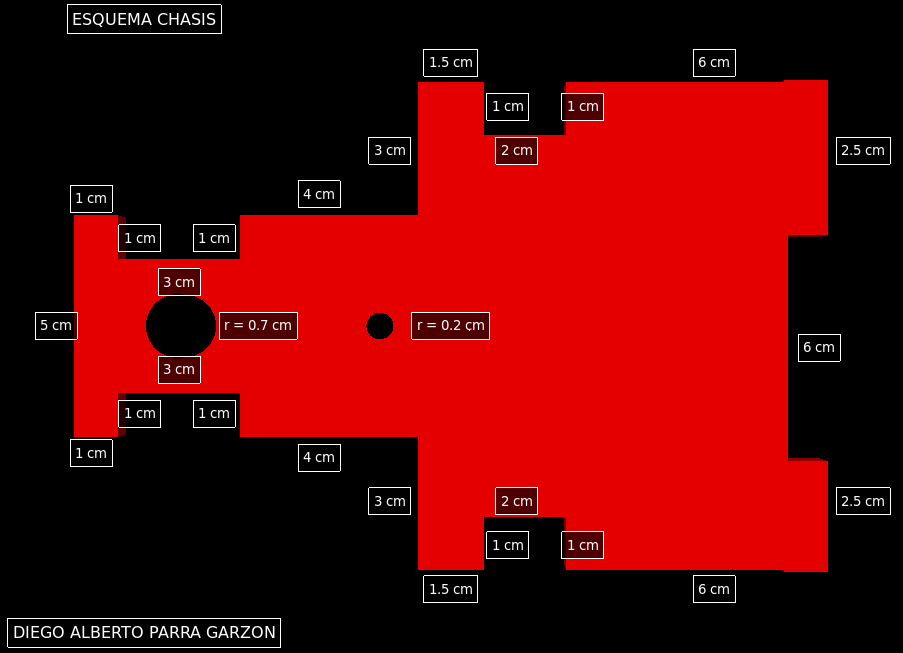
\includegraphics[width=9cm, height=5.7cm]{img/chasis.png} 
\captionof{figure}{En esta figura se observan las dimensiones del chasis que va servir de base del circuito eléctrico y donde reposara el sistema de transmisión del proyecto. Esta figura fue modelada en python visual.}
\label{fig:g7}
\end{Figure}
\vspace{0.6 cm}
Ahora colocamos las llantas del vehículo para esto colocamos dos llantas de 1.5 cm de radio en el eje delantero y luego colocamos dos llantas de 2.5 cm de radio en los ejes traseros; esto con el fin de reducir la rapidez angular de las llantas, la cual se manifestara en una disminución significativa de la rapidez del vehículo.\\\\
Después de tener todo montado como se aprecia en la figura 9, hemos terminado toda la parte del montaje del modulo motorizado.\\\\

\begin{Figure}	
\center
\begin{tabular}{|l|r|}
\hline
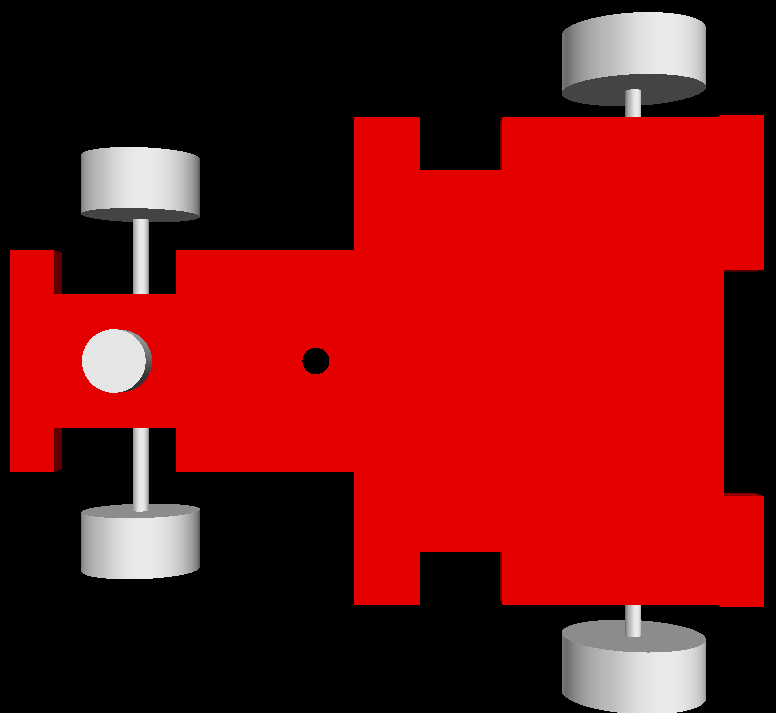
\includegraphics[width=4cm, height=4cm]{img/montaje1.png} & 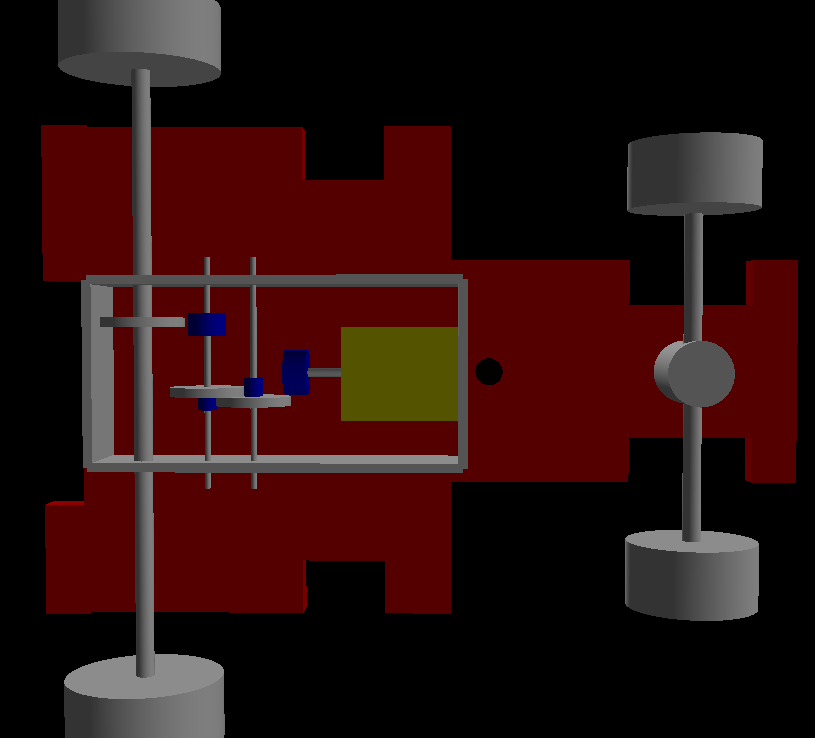
\includegraphics[width=4cm, height=4cm]{img/montaje2.png} \\ \hline
8.A. & 8.B. \\ \hline
\end{tabular}
\captionof{figure}{En la figura 8.A. se muestra la vista superior del montaje del vehículo motorizado, solo falta colocar la parte eléctrica. En la figura 8.B se muestra el montaje del vehículo motorizado con una vista inferior, junto al sistema de transmisión, y el rodamiento delantero. Las figuras fueron modeladas en python visual.}
\label{fig:g8}
\end{Figure}
\vspace{0.6 cm}

Este vehículo se encuentra en una etapa alpha, de esta manera hace falta montar toda la parte estética del vehículo, esto se deja a disposición de cada persona, pues lo realmente importante del vehículo es sus funciones, pero no hay que olvidar que la parte estética es y sera muy importante si este producto quisiera comercializarse.  \\\\

\begin{Figure}	
\center
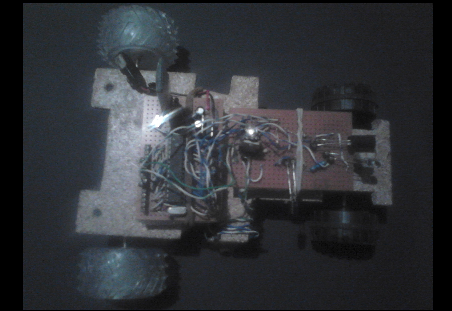
\includegraphics[width=9cm, height=5.7cm]{img/cap6.png} 
\captionof{figure}{Este es el montaje final del vehiculo motorizado.}
\label{fig:g9}
\end{Figure}
\vspace{0.6 cm}

\section{Experiencia de laboratorio}

Una vez descargado nuestro repositorio del proyecto, y teniendo listo el montaje del mismo, es necesario hacer las respectivas pruebas de rapidez e intensidad de radiación del vehículo, para poder realizar estos análisis fue necesario crear una interfaz gráfica en python\cite{PYTHON} que fuera capaz de controlar el  vehículo, obtener datos de este y hacer sus respectivos análisis.\\\\
{\bf{3.1 Pruebas de rapidez}} \\\\
Lo primero que debemos hacer es desde una terminal dirigirnos hasta la carpeta donde hemos descargado nuestro repositorio, luego escribimos cd “Modulo\_Motorizado/2. Interfaz/2.2 Grafica”; ahora escribimos python Gverificar.py  y oprimimos enter, nos debe aparecer la interfaz gráfica de bienvenida, en la que encontraremos una imagen con nuestro vehículo, damos click en la imagen e inmediatamente se nos abrirá otra ventana en donde encontraremos las opciones que necesitamos, damos click en la opción que dice prueba 1, esto nos abrirá otra ventana en la que nos pide la ruta al dispositivo, para esto  escribimos en la terminal blueman-manager, damos al icono de la lupa y nos buscara los dispositivos bluetooth disponibles, apenas veamos nuestro modulo bluetooth, que por lo general siempre aparece como HC-06 o HC-05, damos click derecho sobre este, seleccionamos la opción de emparejar y escribimos la clave de paso, por default es 1234; ahora una vez emparejado procedemos hacer click derecho nuevamente sobre el dispositivo y damos click en la opción “dev B”, si todo sale bien nos dará vía libre al puerto serial y nos dirá la ruta al dispositivo; una vez tengamos el nombre de la ruta al dispositivo la escribimos en la ventana de nuestro programa y damos enter\footnote{Ver figura 10.}, a lo que nos aparecerá, múltiples opciones  para calibrar la rapidez a la que se mueve nuestro modulo. En la primera parte nos aparece las opciones de rapidez sin pausa, por lo que al dar click en cualquiera de estas opciones sin pausa el vehículo se moverá durante 5 segundos a lo que debemos medir la distancia que se desplazo el vehículo, esto lo debemos hacer con cada una de las opciones y de esta manera saber cual es la rapidez a la que se mueve nuestro vehículo. Acto seguido nos aparece las opciones de rapidez con pausa, en esta parte el vehículo se moverá pausadamente 20 veces, por lo que debemos medir la distancia final del vehículo y dividir esta distancia por el numero de veces que se movió, de esta manera conseguimos el desplazamiento en cada pausa. 


\begin{Figure}	
\center
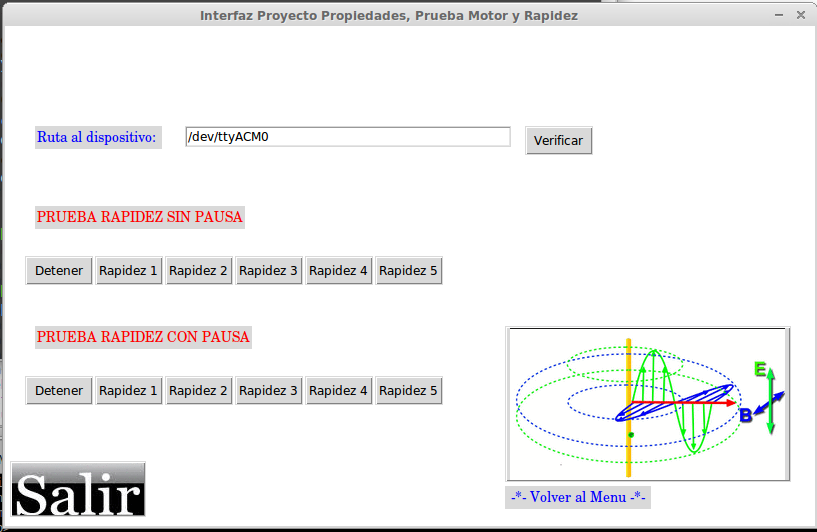
\includegraphics[width=9cm, height=5.7cm]{img/prueba1.png} 
\captionof{figure}{Este es el programa para realizar las pruebas de rapidez con y sin pausa.}
\label{fig:g10}
\end{Figure}
\vspace{0.6 cm}

{\bf{3.2 Pruebas sensor lateral}}\\\\
Una vez terminada la prueba de rapidez en el vehículo, damos click en la imagen de una onda electromagnética, luego oprimimos en el botón que dice prueba 2, una vez allí volvemos a colocar la ruta a nuestro dispositivo, que es la misma que la prueba 1; damos click y nos aparecen dos pruebas una con rapidez sin pausa y otra de rapidez con pausa; el principio que utilizamos aquí es el de electro-recepción pasiva\cite{CIRCUITOS}, pues nuestro diodo receptor\cite{INFRARED} solo esta recibiendo la radiación y este a su vez se comporta como un  transductor\cite{CIRCUITOS}, pues convierte nuestra radiación electromagnética\footnote{Parte clásica.} o los fotones\footnote{Parte cuántica.}, en electricidad, que es interpretada  por nuestro microcontrolador como aumento en la corriente en uno de sus pines receptores análogos,  causando una diferencia de potencial\cite{CIRCUITOS}, con esta diferencia de potencial se trabajara para calibrar nuestro instrumento y poder hacer de el lo más confiable que se pueda en cuanto a sus mediciones refiere.\\\\

\begin{Figure}	
\center
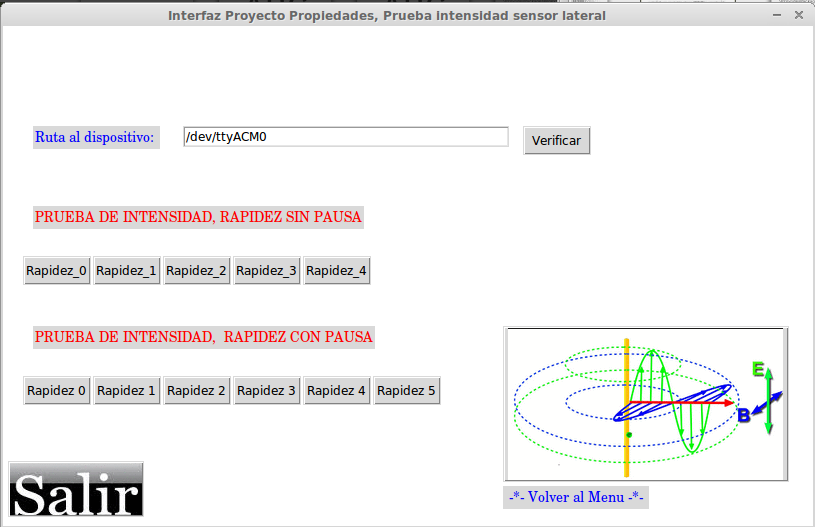
\includegraphics[width=9cm, height=5.7cm]{img/prueba2.png} 
\captionof{figure}{Este es el programa para realizar las pruebas del sensor lateral.}
\label{fig:g11}
\end{Figure}
\vspace{0.6 cm}

Para realizar la prueba de rapidez sin pausa es necesario un ambiente\footnote{No debe estar presente la luz solar ni ninguna fuente que genere cantidades significativas de radiación infrarroja.} controlado,\footnote{Una temperatura ambiente inferior a los 18 $C^{0}$, las hojas de datos de estas piezas electrónicas indican que a temperaturas superiores la corriente no es lineal.} ahora lo primero sera medir la cantidad de datos que es capaz de procesar nuestro ordenador por segundo, para esto oprimimos el botón de rapidez 0 y cambiamos a la ventana de la terminal que esta ejecutando el programa, una vez allí el programa empezara hacer una medición del tiempo que tarda nuestro ordenador en procesar 200 datos\footnote{Para mayor información de esta parte, favor oprimir el botón de ayuda del programa.}, este resultado aparece en nuestra terminal\footnote{El programa va calibrado para trabajar en un ordenador toshiba satellite de 4 Gb de ram.}, mientras captura los datos los gráfica en tiempo real\footnote{Esta parte del código fue creada por mi al no tener un graficador en tiempo real para el puerto serial en GNU-Linux con python.};  una vez hecho esto cerramos la gráfica y cambiamos algunas partes del código\footnote{Ver la sección ayuda del proyecto.} para medir nuevamente  la distancia a la que se desplaza nuestro vehículo después de un tiempo prudencial y de esta manera obtener la rapidez a la que se desplaza nuestro modulo,  ahora es necesario volver a cambiar nuestro código\footnote{Ver sección ayuda del proyecto.}, esto con el fin de obtener unos buenos datos, por ultimo el programa nos mostrara la cantidad de ruido que interfiere en el experimento.  \\\\
Ahora hacemos lo mismo con la parte de rapidez con pausa\footnote{Ver sección ayuda del proyecto.}.\\

{\bf{3.3 Pruebas dispositivo frontal}}\\

Una vez terminada la prueba 2, damos click en la imagen de una onda electromagnética, luego oprimimos en el botón que dice prueba 3, una vez allí volvemos a colocar la ruta a nuestro dispositivo, que es la misma que la prueba 2; damos click y nos aparecen dos pruebas una con rapidez sin pausa y otra de rapidez con pausa; el principio que utilizamos aquí es el de electro-recepción activa\cite{CIRCUITOS}, este consiste en enviar una señal, y luego por las propiedades\cite{BERKELEY} de reflexión\cite{HECHT}, absorción\cite{HECHT}, atenuación\cite{HECHT}, esta llega a nuestro diodo receptor\cite{INFRARED}, osea que es necesario enviar energía, para que esta vaya y vuelva rebotando de los obstáculos a nuestro sensor y este a su vez se comporta como un  transductor\cite{CIRCUITOS}, pues convierte nuestra radiación electromagnética\footnote{Parte clásica.} o los fotones\footnote{Parte cuántica.}, en electricidad, que es interpretada  por nuestro microcontrolador como aumento en la corriente en uno de sus pines receptores análogos,  causando una diferencia de potencial\cite{CIRCUITOS}, con esta diferencia de potencial se trabajara para calibrar nuestro instrumento y poder hacer de el lo más confiable que se pueda en cuanto a sus mediciones refiere.

\begin{Figure}	
\center
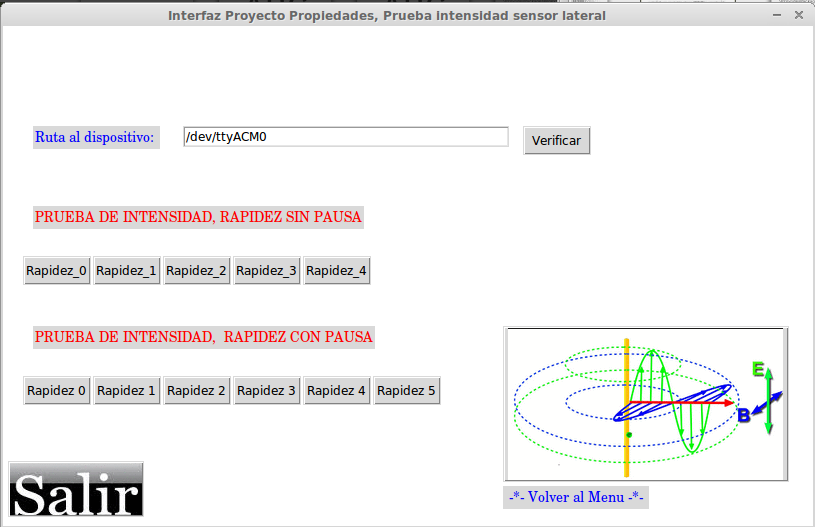
\includegraphics[width=9cm, height=5.7cm]{img/prueba2.png} 
\captionof{figure}{Este es el programa para realizar las pruebas del sensor lateral.}
\label{fig:g11}
\end{Figure}
\vspace{0.4 cm}

Para realizar la prueba de rapidez sin pausa es necesario un ambiente\footnote{No debe estar presente la luz solar ni ninguna fuente que genere cantidades significativas de radiación infrarroja.} controlado,\footnote{Una temperatura ambiente inferior a los 18 $C^{0}$, las hojas de datos de estas piezas electrónicas indican que a temperaturas superiores la corriente no es lineal.} ahora lo primero sera medir la cantidad de datos que es capaz de procesar nuestro ordenador por segundo, para esto oprimimos el botón de rapidez 0 y cambiamos a la ventana de la terminal que esta ejecutando el programa, una vez allí el programa empezara hacer una medición del tiempo que tarda nuestro ordenador en procesar 200 datos\footnote{Para mayor información de esta parte, favor oprimir el botón de ayuda del programa.}, este resultado aparece en nuestra terminal\footnote{El programa va calibrado para trabajar en un ordenador toshiba satellite de 4 Gb de ram.}, mientras captura los datos los gráfica en tiempo real\footnote{Esta parte del código fue creada por mi al no tener un graficador en tiempo real para el puerto serial en GNU-Linux con python.};  una vez hecho esto cerramos la gráfica y cambiamos algunas partes del código\footnote{Ver la sección ayuda del proyecto.} para medir nuevamente  la distancia a la que se desplaza nuestro vehículo después de un tiempo prudencial y de esta manera obtener la rapidez a la que se desplaza nuestro modulo,  ahora es necesario volver a cambiar nuestro código\footnote{Ver sección ayuda del proyecto.}, esto con el fin de obtener unos buenos datos, por ultimo el programa nos mostrara la cantidad de ruido que interfiere en el experimento.  \\\\
Ahora hacemos lo mismo con la parte de rapidez con pausa\footnote{Ver sección ayuda del proyecto.}.

\section{Analisis de resultados}
{\bf{4.1 Análisis de la Prueba 1}}\\\\
Después de cerca de 100 mediciones en cada una de las opciones de esa sección del proyecto se llegan a las siguientes conclusiones: \\\\
{\bf{4.1.1 Rapidez sin pausa}}\\

En la tabla 1 se puede apreciar los resultados de la prueba de rapidez sin pausa en cada opción del programa, se trabaja con un corriente menor que la salida del pin analógico que es de 35 mA.\\\\
El error en la medida de los datos de rapidez es la misma que nos ofrece nuestro instrumento de medición que en este caso es un metro cuyo error es $\frac{+}{-} 1 mm$, el error en la medida de la corriente es de $\frac{+}{-} 1 mA$.\\

\begin{tabular}{|l|c|c|} 
\hline
\bf{Opción} &  \bf{Rapidez $(\frac{m}{s})$} & \bf{Corriente (mA)}\\
\hline
Rapidez 1 & 0.103 & 20 \\
\hline
Rapidez 2 & 0.130 & 23 \\
\hline
Rapidez 3 & 0.138 & 24 \\
\hline 
Rapidez 4 & 0.154 & 25 \\
\hline
\end{tabular}
\\
\textbf{Tabla 1.} Datos obtenidos de la Prueba 1, rapidez sin pausa, la corrientes es la que circula por el motor con cada opción. \\

{\bf{4.1.2 Rapidez con pausa}} \\
En la tabla 2 se puede apreciar los resultados de la prueba de rapidez con pausa en cada opción del programa, se trabaja con un corriente menor que la salida del pin analógico que es de 35 mA.\\\\
El error en la medida de los datos de rapidez es la misma que nos ofrece nuestro instrumento de medición que en este caso es un metro cuyo error es $\frac{+}{-} 1 mm$, no se calcula la corriente pues varia demasiado rapido para ser medida.\\

\begin{tabular}{|l|c|c|} 
\hline
\bf{Opción} & Distancia final (cm) & Avance (cm)\\
\hline
Rapidez 1 & 9 &0.45 \\
\hline
Rapidez 2 & 8 &0.4 \\
\hline
Rapidez 3 & 6.5 &0.325 \\
\hline 
Rapidez 4 & 6 & 0.3 \\
\hline
\end{tabular}
\\
\textbf{Tabla 2.} Datos obtenidos de la Prueba 1, rapidez con pausa, la distancia final es la distancia después de 20 repeticiones, y la distancia de avance es la distancia final dividida 20 repeticiones. \\

{\bf{4.2 Sensor lateral}} \\\\
{\bf{4.2.1 Rapidez sin pausa}}\\\\
En la tabla 1 se puede apreciar los resultados de la prueba de rapidez sin pausa en cada opción del programa, se trabaja con un corriente menor que la salida del pin analógico que es de 35 mA.\\\\
El error en la medida de los datos de rapidez es la misma que nos ofrece nuestro instrumento de medición que en este caso es un metro cuyo error es $\frac{+}{-} 1 mm$, el error en la medida de la corriente es de $\frac{+}{-} 1 mA$.\\







\begin{thebibliography}{99}
\bibitem{ARDUINO} Arduino, pagina oficial, proyecto arduino. http://www.arduino.cc/
\bibitem{REGULADOR} Hoja de datos  transistor lm 7805CV. http://pdf.datasheetcatalog.net/datasheet/fairchild/\\LM7805.pdf
\bibitem{TIP122} Hoja de datos del transistor tip 122. http://pdf.datasheetcatalog.net/datasheet/fairchild/\\TIP122.pdf.
\bibitem{DIODO}  Hoja de datos diodo regulador 1N4001. http://pdf.datasheetcatalog.net/datasheet/lrc/\\1N4001.pdf
\bibitem{INFRARED} Hoja de datos de los diodos led infrarrojos, emisor y receptor. \\ http://www.datasheetarchive.com/dlmain/Datasheets\\-31/DSA-617614.pdf
\bibitem{FRITZING} Pagina oficial del proyecto fritzing http://fritzing.org/home/ 
\bibitem{PYTHON} Notas del curso, python para el computo científico, curso de actualización académica de la DGAPA-UNAM, Facultad de ciencias, Dr. David P. Sanders, 5 de agosto de 2013. 
\bibitem{CIRCUITOS} Fundamentos de circuitos eléctricos, tercera edición, editorial Mc Graw Hill, Charles K. Alexander and Matthew N. O. Sadiku. 
\bibitem{BERKELEY} Berkeley Physics Course, volumen 3, Ondas (Crawford).
\bibitem{HECHT} Óptica, Eugene Hecht, tercera edición
\end{thebibliography}
\end{multicols}
\end{document}




